% Options for packages loaded elsewhere
\PassOptionsToPackage{unicode}{hyperref}
\PassOptionsToPackage{hyphens}{url}
\PassOptionsToPackage{dvipsnames,svgnames,x11names}{xcolor}
%
\documentclass[
  11pt,
  letterpaper,
]{article}
\usepackage{amsmath,amssymb}
\usepackage{iftex}
\ifPDFTeX
  \usepackage[T1]{fontenc}
  \usepackage[utf8]{inputenc}
  \usepackage{textcomp} % provide euro and other symbols
\else % if luatex or xetex
  \usepackage{unicode-math} % this also loads fontspec
  \defaultfontfeatures{Scale=MatchLowercase}
  \defaultfontfeatures[\rmfamily]{Ligatures=TeX,Scale=1}
\fi
\usepackage{lmodern}
\ifPDFTeX\else
  % xetex/luatex font selection
\fi
% Use upquote if available, for straight quotes in verbatim environments
\IfFileExists{upquote.sty}{\usepackage{upquote}}{}
\IfFileExists{microtype.sty}{% use microtype if available
  \usepackage[]{microtype}
  \UseMicrotypeSet[protrusion]{basicmath} % disable protrusion for tt fonts
}{}
\makeatletter
\@ifundefined{KOMAClassName}{% if non-KOMA class
  \IfFileExists{parskip.sty}{%
    \usepackage{parskip}
  }{% else
    \setlength{\parindent}{0pt}
    \setlength{\parskip}{6pt plus 2pt minus 1pt}}
}{% if KOMA class
  \KOMAoptions{parskip=half}}
\makeatother
\usepackage{xcolor}
\usepackage[margin=1in]{geometry}
\usepackage{longtable,booktabs,array}
\usepackage{calc} % for calculating minipage widths
% Correct order of tables after \paragraph or \subparagraph
\usepackage{etoolbox}
\makeatletter
\patchcmd\longtable{\par}{\if@noskipsec\mbox{}\fi\par}{}{}
\makeatother
% Allow footnotes in longtable head/foot
\IfFileExists{footnotehyper.sty}{\usepackage{footnotehyper}}{\usepackage{footnote}}
\makesavenoteenv{longtable}
\usepackage{graphicx}
\makeatletter
\def\maxwidth{\ifdim\Gin@nat@width>\linewidth\linewidth\else\Gin@nat@width\fi}
\def\maxheight{\ifdim\Gin@nat@height>\textheight\textheight\else\Gin@nat@height\fi}
\makeatother
% Scale images if necessary, so that they will not overflow the page
% margins by default, and it is still possible to overwrite the defaults
% using explicit options in \includegraphics[width, height, ...]{}
\setkeys{Gin}{width=\maxwidth,height=\maxheight,keepaspectratio}
% Set default figure placement to htbp
\makeatletter
\def\fps@figure{htbp}
\makeatother
\setlength{\emergencystretch}{3em} % prevent overfull lines
\providecommand{\tightlist}{%
  \setlength{\itemsep}{0pt}\setlength{\parskip}{0pt}}
\setcounter{secnumdepth}{-\maxdimen} % remove section numbering
% definitions for citeproc citations
\NewDocumentCommand\citeproctext{}{}
\NewDocumentCommand\citeproc{mm}{%
  \begingroup\def\citeproctext{#2}\cite{#1}\endgroup}
\makeatletter
 % allow citations to break across lines
 \let\@cite@ofmt\@firstofone
 % avoid brackets around text for \cite:
 \def\@biblabel#1{}
 \def\@cite#1#2{{#1\if@tempswa , #2\fi}}
\makeatother
\newlength{\cslhangindent}
\setlength{\cslhangindent}{1.5em}
\newlength{\csllabelwidth}
\setlength{\csllabelwidth}{3em}
\newenvironment{CSLReferences}[2] % #1 hanging-indent, #2 entry-spacing
 {\begin{list}{}{%
  \setlength{\itemindent}{0pt}
  \setlength{\leftmargin}{0pt}
  \setlength{\parsep}{0pt}
  % turn on hanging indent if param 1 is 1
  \ifodd #1
   \setlength{\leftmargin}{\cslhangindent}
   \setlength{\itemindent}{-1\cslhangindent}
  \fi
  % set entry spacing
  \setlength{\itemsep}{#2\baselineskip}}}
 {\end{list}}
\usepackage{calc}
\newcommand{\CSLBlock}[1]{\hfill\break\parbox[t]{\linewidth}{\strut\ignorespaces#1\strut}}
\newcommand{\CSLLeftMargin}[1]{\parbox[t]{\csllabelwidth}{\strut#1\strut}}
\newcommand{\CSLRightInline}[1]{\parbox[t]{\linewidth - \csllabelwidth}{\strut#1\strut}}
\newcommand{\CSLIndent}[1]{\hspace{\cslhangindent}#1}
\ifLuaTeX
\usepackage[bidi=basic]{babel}
\else
\usepackage[bidi=default]{babel}
\fi
\babelprovide[main,import]{spanish}
% get rid of language-specific shorthands (see #6817):
\let\LanguageShortHands\languageshorthands
\def\languageshorthands#1{}
\ifLuaTeX
  \usepackage{selnolig}  % disable illegal ligatures
\fi
\usepackage{bookmark}
\IfFileExists{xurl.sty}{\usepackage{xurl}}{} % add URL line breaks if available
\urlstyle{same}
\hypersetup{
  pdftitle={Tecnologías cuánticas como infraestructura estratégica: evidencia, rutas de adopción y una agenda nacional de investigación para 2025-2035},
  pdfauthor={Edgar Valdés, Hadox Research Labs},
  pdflang={es-MX},
  colorlinks=true,
  linkcolor={blue},
  filecolor={blue},
  citecolor={blue},
  urlcolor={blue},
  pdfcreator={LaTeX via pandoc}}

\title{Tecnologías cuánticas como infraestructura estratégica:
evidencia, rutas de adopción y una agenda nacional de investigación para
2025-2035\thanks{Preparado para el track de Tecnologías Cuánticas de la
vigésima tercera edición de la Conferencia Anual de la Global
Information Technology Management Association, Monterrey, México, 6-8 de
mayo de 2026, en la cual Edgar Antonio Valdés Porras participa como
Track Chair. El autor agradece a Rogelio Marín y al Centro de
Investigación en Matemáticas, A.C. por el apoyo intelectual y el
contexto institucional. Todas las interpretaciones y errores remanentes
son responsabilidad del autor.}}
\author{Edgar Valdés, Hadox Research Labs}
\date{Abril de 2026}

\begin{document}
\maketitle

\section{Resumen}\label{resumen}

Las tecnologías cuánticas han pasado de ser un programa
predominantemente científico a constituir un dominio de infraestructura
estratégica que afecta la computación, la sensórica, las comunicaciones,
la ciberseguridad, la investigación industrial y la política nacional de
innovación. Este artículo examina el horizonte de adopción 2025-2035
mediante una síntesis integradora de la literatura en ciencia de la
información cuántica, teoría de sistemas de innovación, investigación
sobre adopción empresarial, datos de estrategias nacionales de la OCDE,
mapeo de patentes OCDE-OEP, indicadores bibliométricos de OpenAlex,
estándares del NIST, estudios sobre integración con cómputo de alto
desempeño (HPC) y encuestas de preparación institucional. El análisis
muestra que la adopción cuántica no es una transición de mercado única,
sino una transición estratificada de capacidades: la criptografía
post-cuántica y ciertas aplicaciones de sensórica cuántica ya poseen
relevancia institucional; la comunicación cuántica avanza mediante redes
especializadas y bancos de prueba de seguridad; y la computación
cuántica de propósito general sigue dependiendo de la corrección de
errores, la economía de qubits lógicos, la evaluación comparativa a
nivel de aplicación, la integración híbrida cuántico-clásica y la
capacidad de acoplar unidades de procesamiento cuántico a entornos HPC.
La evidencia empírica revela aceleración, pero también desigualdad
estructural. Para octubre de 2025, los gobiernos habían anunciado
compromisos públicos cuánticos por aproximadamente USD 55.7 mil
millones; Fundstat de la OCDE identificó USD 11.235 mil millones PPP en
12,209 apoyos de I+D relacionados con tecnologías cuánticas durante
2015-2023; el mapeo OCDE-OEP identificó 31,700 familias de patentes
cuánticas entre 2005 y 2024; y la bibliometría de OpenAlex muestra una
geografía de publicaciones concentrada en Estados Unidos, China,
Alemania, Reino Unido y Francia. Estos hallazgos apoyan un
desplazamiento desde métricas de preparación centradas en hardware hacia
la capacidad de absorción: la capacidad de empresas y Estados para
entender, probar, comparar, adquirir, asegurar, regular y eventualmente
producir tecnologías cuánticas. El artículo concluye con una hoja de
ruta por etapas, una crítica de errores comunes de adopción y una agenda
de investigación de frontera para naciones que buscan soberanía
tecnológica de largo plazo.

\textbf{Palabras clave:} tecnologías cuánticas, computación cuántica,
sensórica cuántica, criptografía post-cuántica, comunicación cuántica,
sistemas nacionales de innovación, capacidad de absorción, política
cuántica, infraestructura estratégica

\section{1. Introducción}\label{introducciuxf3n}

El término ``tecnología cuántica'' tiene hoy dos significados distintos.
En el discurso público suele usarse como sinónimo de computación
cuántica, acompañado de afirmaciones según las cuales los procesadores
cuánticos transformarán pronto todo problema computacional. En la
literatura de investigación, en cambio, designa una familia más amplia
de tecnologías que explotan estados cuánticos controlados para
computación, medición, comunicación, simulación, temporización y
seguridad (\citeproc{ref-dowling2003}{Dowling y Milburn 2003};
\citeproc{ref-acin2018}{Acin et~al. 2018}). Esta distinción es
analíticamente decisiva porque modifica la forma en que se evalúan la
adopción, la política pública, la inversión y la estrategia nacional.

La primera revolución cuántica produjo tecnologías como transistores,
láseres, imagen por resonancia magnética, electrónica de semiconductores
y relojes atómicos. Estos dispositivos usaban la teoría cuántica de
forma indirecta, a menudo mediante propiedades estadísticas o colectivas
de la materia. La segunda revolución cuántica es distinta porque busca
la ingeniería directa de estados cuánticos individuales o colectivos,
incluyendo superposición, entrelazamiento, compresión cuántica,
tunelamiento y retroacción de medición
(\citeproc{ref-dowling2003}{Dowling y Milburn 2003};
\citeproc{ref-giovannetti2011}{Giovannetti, Lloyd, y Maccone 2011}). Por
ello, las tecnologías cuánticas se ubican en la frontera entre física e
infraestructura. Son instrumentos científicos, pero también componentes
futuros de la ciberseguridad, las finanzas, las telecomunicaciones, la
energía, la medicina, la logística, el descubrimiento de materiales, la
defensa y la administración pública.

El análisis trata las tecnologías cuánticas como infraestructura
estratégica. Este encuadre tiene tres implicaciones. Primero, las
tecnologías cuánticas no constituyen un solo mercado de productos;
forman una pila de capacidades científicas, industriales, de software,
seguridad, metrología y gobernanza. Segundo, su valor económico no será
capturado simplemente por los primeros proveedores ni por los anuncios
de hardware más grandes. Será capturado por organizaciones y países que
desarrollen la capacidad de evaluar afirmaciones cuánticas, integrar
herramientas cuánticas con sistemas clásicos y adaptar compras públicas,
estándares, talento y ciberseguridad. Tercero, las acciones más
importantes de corto plazo no siempre son las que suenan más futuristas.
La criptografía post-cuántica (PQC), las compras públicas cuánticamente
seguras, los pilotos de sensórica cuántica, la metrología, la formación
de fuerza laboral y la experimentación mediada por la nube pueden
producir más valor estratégico antes de que llegue la computación
cuántica universal tolerante a fallas.

Seis preguntas de investigación estructuran el análisis.

\begin{enumerate}
\def\labelenumi{\arabic{enumi}.}
\tightlist
\item
  ¿Qué implica la literatura académica sobre la madurez y las rutas de
  adopción de la computación cuántica, la sensórica, la comunicación y
  la criptografía post-cuántica?
\item
  ¿Qué indicadores cuantitativos pueden usarse para estimar la
  preparación cuántica global cuando los datos directos de adopción
  siguen incompletos?
\item
  ¿Cómo modifica el cómputo de alto desempeño la ruta de adopción de la
  computación cuántica?
\item
  ¿Cómo pueden las naciones y las empresas comparar tecnologías
  cuánticas bajo condiciones de incertidumbre técnica, exageración
  comercial y competencia geopolítica?
\item
  ¿Cuáles son las principales barreras para la adopción cuántica entre
  2025 y 2035?
\item
  ¿Qué hoja de ruta puede guiar a una nación hacia capacidades cuánticas
  sin encierro prematuro en hardware inmaduro ni política de innovación
  puramente retórica?
\end{enumerate}

El argumento es deliberadamente crítico. Las tecnologías cuánticas son
reales y estratégicamente importantes, pero su adopción suele discutirse
con evidencia débil. Los pronósticos de mercado pueden ser señales
útiles, pero no son datos de adopción. El conteo de qubits no equivale a
capacidad de sistema. La ventaja en circuitos aleatorios no implica
automáticamente valor comercial. La distribución cuántica de claves no
reemplaza de forma universal a la criptografía post-cuántica. El
aprendizaje automático cuántico no es automáticamente superior al
aprendizaje automático clásico. Una estrategia nacional creíble requiere
separar con claridad la posibilidad científica, la factibilidad de
ingeniería, la preparación organizacional y el valor público.

\section{2. Revisión de literatura y marco
teórico}\label{revisiuxf3n-de-literatura-y-marco-teuxf3rico}

\subsection{2.1 De la revolución cuántica a la
infraestructura}\label{de-la-revoluciuxf3n-cuuxe1ntica-a-la-infraestructura}

La agenda moderna de tecnología cuántica comienza con la afirmación de
que los sistemas cuánticos individuales pueden ser diseñados como
recursos, en vez de tratarse como fenómenos microscópicos inevitables.
Dowling y Milburn (\citeproc{ref-dowling2003}{2003}) describieron este
proceso como la segunda revolución cuántica. La hoja de ruta cuántica
europea organizó posteriormente el campo en comunicación cuántica,
computación cuántica, simulación cuántica, metrología y sensórica
cuánticas, control cuántico y software cuántico
(\citeproc{ref-acin2018}{Acin et~al. 2018}). Esta taxonomía sigue siendo
útil, pero la estrategia nacional requiere una clasificación adicional
por preparación para la adopción, carga infraestructural, urgencia de
seguridad y dependencia de tolerancia a fallas.

La computación cuántica recibe la mayor atención porque sus
implicaciones computacionales de largo plazo son profundas. Montanaro
(\citeproc{ref-montanaro2016}{2016}) muestra que los algoritmos
cuánticos pueden ofrecer aceleraciones en clases específicas de
problemas, como búsqueda, optimización, simulación, sistemas lineales y
criptografía. Preskill (\citeproc{ref-preskill2018}{2018}) caracterizó
la era actual como computación cuántica ruidosa de escala intermedia, en
la cual los dispositivos son lo suficientemente grandes para ser
científicamente interesantes, pero demasiado ruidosos para muchos
algoritmos tolerantes a fallas. Bharti et~al.
(\citeproc{ref-bharti2022}{2022}) y Cerezo et~al.
(\citeproc{ref-cerezo2021}{2021}) muestran que el paisaje algorítmico de
corto plazo está dominado por métodos variacionales e híbridos
cuántico-clásicos, no por la ejecución madura de algoritmos tolerantes a
fallas a escala de Shor. Esto importa porque la ruta desde el
dispositivo de laboratorio hasta la ventaja operativa no es lineal: pasa
por corrección de errores, diseño de benchmarks, herramientas de
software y validación específica por aplicación.

La simulación cuántica y la química cuántica ofrecen el caso intelectual
más claro para la computación cuántica futura porque los sistemas
objetivo son, ellos mismos, mecánico-cuánticos. Georgescu, Ashhab, y
Nori (\citeproc{ref-georgescu2014}{2014}) presentan la simulación
cuántica como una clase natural de aplicaciones, mientras que Cao et~al.
(\citeproc{ref-cao2019}{2019}) y Bauer et~al.
(\citeproc{ref-bauer2020}{2020}) revisan algoritmos para química y
ciencia de materiales. Aun aquí, sin embargo, la ventaja teórica no
resuelve el problema de adopción. Los flujos de trabajo útiles requieren
precisión química, codificación del problema, mitigación o corrección de
errores, validación contra experimentos e integración con pipelines de
investigación existentes.

La sensórica cuántica sigue una ruta distinta. Degen, Reinhard, y
Cappellaro (\citeproc{ref-degen2017}{2017}) definen la sensórica
cuántica como el uso de sistemas cuánticos para medir magnitudes físicas
con alta sensibilidad. Giovannetti, Lloyd, y Maccone
(\citeproc{ref-giovannetti2011}{2011}) y Pezze et~al.
(\citeproc{ref-pezze2018}{2018}) muestran por qué el entrelazamiento y
los estados no clásicos pueden mejorar la metrología. Aplicaciones como
relojes, magnetómetros, gravímetros, sensores inerciales, navegación,
geodesia y sensórica biomédica no requieren computación cuántica
universal tolerante a fallas. Esto convierte a la sensórica en un
dominio de adopción más cercano, aunque sus requisitos de ingeniería
siguen siendo exigentes: robustecimiento, calibración, costo,
estabilidad ambiental, despliegue en campo e integración con flujos de
trabajo de dominio.

La comunicación cuántica también posee un perfil de madurez distinto.
Kimble (\citeproc{ref-kimble2008}{2008}) y Wehner, Elkouss, y Hanson
(\citeproc{ref-wehner2018}{2018}) describen el internet cuántico como
una red futura para distribución de entrelazamiento, comunicación
segura, sensórica distribuida y, eventualmente, computación cuántica
distribuida. Pirandola et~al. (\citeproc{ref-pirandola2020}{2020}) y Xu
et~al. (\citeproc{ref-xu2020}{2020}) revisan la criptografía cuántica y
QKD con dispositivos realistas. El caso de investigación es sólido, pero
el despliegue práctico enfrenta límites de distancia, pérdida,
autenticación, nodos confiables, vulnerabilidades de dispositivos, costo
y estándares. El resultado es una ruta de infraestructura especializada,
no una solución universal de ciberseguridad.

La PQC es conceptualmente distinta de la comunicación cuántica. Es
criptografía clásica diseñada para resistir ataques cuánticos. Bernstein
y Lange (\citeproc{ref-bernstein2017}{2017}) revisan sus fundamentos
técnicos; Mosca (\citeproc{ref-mosca2018}{2018}) encuadra el problema de
ciberseguridad mediante la relación entre vida útil de los datos, tiempo
de migración y horizonte de una computadora cuántica criptográficamente
relevante. Gidney y Ekera (\citeproc{ref-gidney2021}{2021}) muestran por
qué la amenaza no es inminente en sentido operativo pero sí
estratégicamente seria: los estimados para atacar RSA-2048 requieren
máquinas tolerantes a fallas muy grandes, pero el problema de ``capturar
ahora, descifrar después'' empieza antes de que esas máquinas existan.
Esto convierte a la PQC en el dominio de adopción nacional más claro en
el corto plazo.

\subsection{2.2 Teoría de adopción: capacidad de absorción y sistemas
nacionales de
innovación}\label{teoruxeda-de-adopciuxf3n-capacidad-de-absorciuxf3n-y-sistemas-nacionales-de-innovaciuxf3n}

La adopción cuántica no es solo un problema de hardware. Es un problema
de capacidad de absorción. Cohen y Levinthal
(\citeproc{ref-cohen1990}{1990}) definen la capacidad de absorción como
la habilidad para reconocer, asimilar y explotar conocimiento externo.
Las tecnologías cuánticas requieren una capacidad de absorción
inusualmente alta porque son difíciles de evaluar, exigen conocimiento
especializado y dependen de activos complementarios como estándares,
laboratorios, plataformas de software, inventarios criptográficos y
reglas de adquisición.

La teoría de sistemas nacionales de innovación refuerza este punto. El
desempeño tecnológico depende de redes de universidades, empresas,
agencias públicas, organismos de estandarización, instituciones
financieras y usuarios industriales, no de invenciones aisladas
(\citeproc{ref-lundvall1992}{Lundvall 1992};
\citeproc{ref-nelson1993}{Nelson 1993}). La política de innovación
orientada por misiones añade que los gobiernos pueden moldear mercados
cuando definen misiones públicas, coordinan capacidades y crean demanda
para tecnologías difíciles (\citeproc{ref-mazzucato2018}{Mazzucato
2018}). Las tecnologías cuánticas se ajustan a este marco porque el
sector privado por sí solo difícilmente financiará toda la ciencia
fundamental, transición de ciberseguridad, estandarización, formación
laboral e infraestructura de testbeds requeridas para la adopción.

La evidencia de adopción empresarial empieza a alcanzar a la física.
Kwon et~al. (\citeproc{ref-kwon2026}{2026}) analizan la intención de
adopción de computación cuántica mediante entrevistas con expertos y una
encuesta a 250 tomadores de decisión de TI. Encuentran que la ventaja
cuántica percibida, la creencia en superioridad cuántica, la asignación
continua de presupuesto, el apoyo regulatorio y la co-creación aumentan
la intención de adopción, mientras que la resistencia organizacional y
el riesgo financiero la reducen. El resultado coincide con la literatura
más amplia sobre difusión de innovaciones: la adopción requiere no solo
promesa tecnológica, sino ventaja relativa, compatibilidad, capacidad de
prueba, recursos organizacionales y apoyo institucional
(\citeproc{ref-rogers2003}{Rogers 2003}).

\subsection{2.3 El error estratégico: confundir hitos científicos con
adopción}\label{el-error-estratuxe9gico-confundir-hitos-cientuxedficos-con-adopciuxf3n}

El campo cuántico ha producido hitos científicos genuinos. Arute et~al.
(\citeproc{ref-arute2019}{2019}) demostraron ventaja computacional
cuántica en un procesador superconductor programable para una tarea de
muestreo. Harrow y Montanaro (\citeproc{ref-harrow2017}{2017}) explican
por qué estas demostraciones importan para la complejidad computacional.
Sin embargo, la ventaja científica y la ventaja económica no son
equivalentes. Una tarea de muestreo de circuitos aleatorios puede
demostrar que un dispositivo cuántico es difícil de simular clásicamente
sin resolver un problema empresarial valioso. Esto no es una crítica a
la ciencia; es una advertencia contra el uso de una inferencia
equivocada para política pública.

La misma distinción aplica al aprendizaje automático cuántico. Biamonte
et~al. (\citeproc{ref-biamonte2017}{2017}) y Schuld y Killoran
(\citeproc{ref-schuld2019}{2019}) identifican mecanismos plausibles para
modelos de aprendizaje cuántico, especialmente mediante mapas de
características y representaciones en espacios de Hilbert. McClean
et~al. (\citeproc{ref-mcclean2018}{2018}), sin embargo, identifican las
mesetas estériles como un obstáculo serio de entrenamiento. Para la
estrategia empresarial, la pregunta relevante no es si un circuito es
cuántico, sino si mejora precisión, tiempo de solución, consumo
energético, robustez, interpretabilidad o costo frente al mejor baseline
clásico.

\section{3. Datos y métodos}\label{datos-y-muxe9todos}

\subsection{3.1 Diseño de
investigación}\label{diseuxf1o-de-investigaciuxf3n}

El estudio se diseña como una síntesis integradora de investigación.
Este diseño es apropiado porque el objeto de análisis no es una sola
estimación empírica, sino una interpretación estratégica de una base de
evidencia heterogénea. El corpus incluye ciencia de la información
cuántica, teoría de innovación, reportes de política pública, datos
bibliométricos abiertos, mapeo de patentes, documentos de estándares y
encuestas de preparación empresarial.

La metodología siguió cuatro pasos. Primero, la literatura se organizó
en siete dominios: computación cuántica, sensórica cuántica,
comunicación cuántica, PQC, integración con cómputo de alto desempeño,
teoría de innovación/adopción y política nacional. Segundo, cada dominio
fue evaluado según preparación tecnológica, barreras de adopción,
requisitos de infraestructura y relevancia para la estrategia nacional.
Tercero, se ensamblaron proxies cuantitativos de adopción a partir de
fuentes de la OCDE, OCDE-OEP, OpenAlex, NIST y encuestas de
preparación.\footnote{Se usan proxies de adopción porque no existen
  datos públicos completos sobre despliegue cuántico directo. Estos
  proxies miden dimensiones distintas de preparación y no se tratan como
  indicadores intercambiables.} Cuarto, la evidencia se tradujo en una
hoja de ruta estratégica y un conjunto de criterios de decisión para
naciones y empresas.

El diseño no es una revisión sistemática en el sentido estrecho de
PRISMA, pues el objetivo no es estimar un tamaño de efecto a través de
estudios empíricos comparables. Es una revisión narrativa estructurada y
una síntesis de evidencia de un campo tecnológico emergente en el cual
la evidencia relevante proviene de física, ciencias de la computación,
ciberseguridad, política pública e investigación en gestión. Los
criterios de inclusión priorizaron artículos de revisión importantes,
trabajos fundacionales altamente citados, estudios empíricos de
adopción, literatura de ciberseguridad relevante para estándares y
datasets recientes de instituciones públicas.

\subsection{3.2 Selección de fuentes}\label{selecciuxf3n-de-fuentes}

El corpus académico se extrajo de revistas y proceedings en física,
ciencias de la computación, ingeniería, criptografía, gestión y política
de innovación. Incluye trabajos publicados en \emph{Reviews of Modern
Physics}, \emph{Nature}, \emph{Nature Reviews Physics}, \emph{Nature
Communications}, \emph{Physical Review Letters}, \emph{Physical Review
A}, \emph{PRX Quantum}, \emph{npj Quantum Information}, \emph{Quantum},
\emph{Chemical Reviews}, \emph{Applied Physics Reviews}, \emph{Annual
Review of Condensed Matter Physics}, \emph{IEEE Transactions on Quantum
Engineering}, \emph{IEEE Security \& Privacy}, \emph{International
Journal of Information Management}, \emph{Administrative Science
Quarterly} e \emph{Industrial and Corporate Change}.

La capa cuantitativa utiliza datasets públicos y fuentes oficiales. El
material de estrategias nacionales de la OCDE aporta estimaciones de
compromisos públicos y modelos de gobernanza. Fundstat de la OCDE aporta
evidencia de apoyos a proyectos. El mapeo OCDE-OEP aporta evidencia de
familias de patentes. OpenAlex aporta proxies de publicaciones y
afiliación por país. NIST, NSA y CISA aportan estándares y orientación
de ciberseguridad. Estas fuentes no se tratan como intercambiables. El
financiamiento mide compromiso estatal; las patentes miden invención y
apropiación; las publicaciones miden capacidad científica de absorción;
los estándares miden preparación institucional; las encuestas miden
preparación organizacional.

\subsection{3.3 Extracción
bibliométrica}\label{extracciuxf3n-bibliomuxe9trica}

Los datos de OpenAlex se extrajeron para 2015-2025 usando los conceptos
``Quantum technology'' (C190463098) y ``Post-quantum cryptography''
(C108277079), agrupados por año de publicación y país institucional. La
consulta de tecnología cuántica devolvió 15,279 trabajos en el conjunto
extraído. Las principales afiliaciones por país fueron Estados Unidos
(2,584), China (1,641), Alemania (1,225), Reino Unido (1,102), Francia
(607), Italia (552), India (551), Japón (519), Canadá (463) y Australia
(438). México apareció con 56 trabajos. La consulta de criptografía
post-cuántica mostró una distribución distinta: Estados Unidos (168),
India (163), China (132), Reino Unido (61), Alemania (60), Japón (52),
Francia (42), Corea (36), España (30) y Rusia (29) encabezaron los
conteos; México apareció con 5 trabajos.

Estos conteos se usan con cautela. La asignación de conceptos en
OpenAlex, los metadatos de afiliación, la coautoría y las prácticas de
indexación afectan los resultados. El conteo de tecnología cuántica de
2025 es especialmente alto frente a años previos; por tanto, la
tendencia anual se interpreta como una señal de consulta e indexación,
no como una medición precisa de producción global anual. Los conteos por
país son más útiles como proxy amplio de capacidad científica de
absorción.

\begin{figure}
\centering
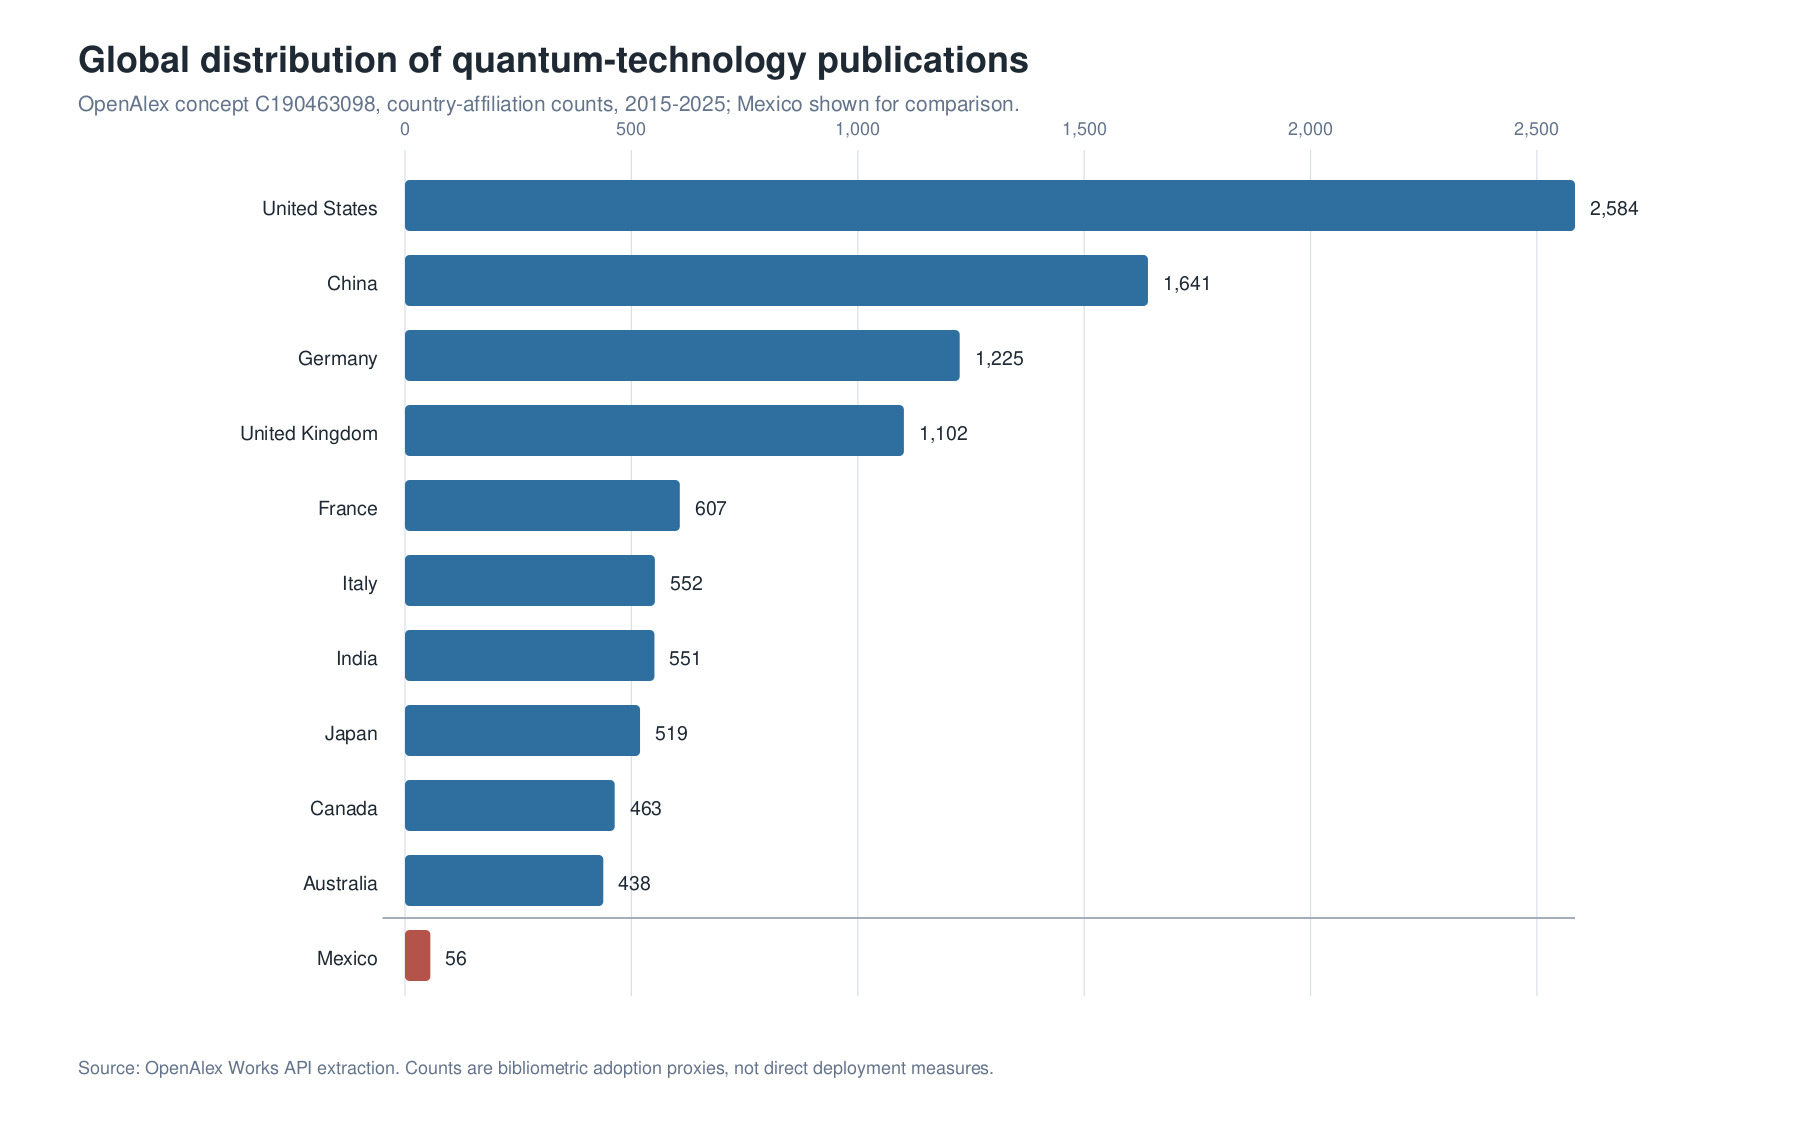
\includegraphics[width=0.95\textwidth,height=\textheight]{figures/fig1_global_country_distribution.png}
\caption{Distribución global de capacidad de publicación en tecnología
cuántica. Los conteos de afiliación por país de OpenAlex para el
concepto ``Quantum technology'' muestran una geografía concentrada
liderada por Estados Unidos, China, Alemania, Reino Unido y Francia, con
México incluido como caso de comparación. Los conteos son proxies
bibliométricos, no medidas directas de despliegue.}
\end{figure}

\begin{figure}
\centering
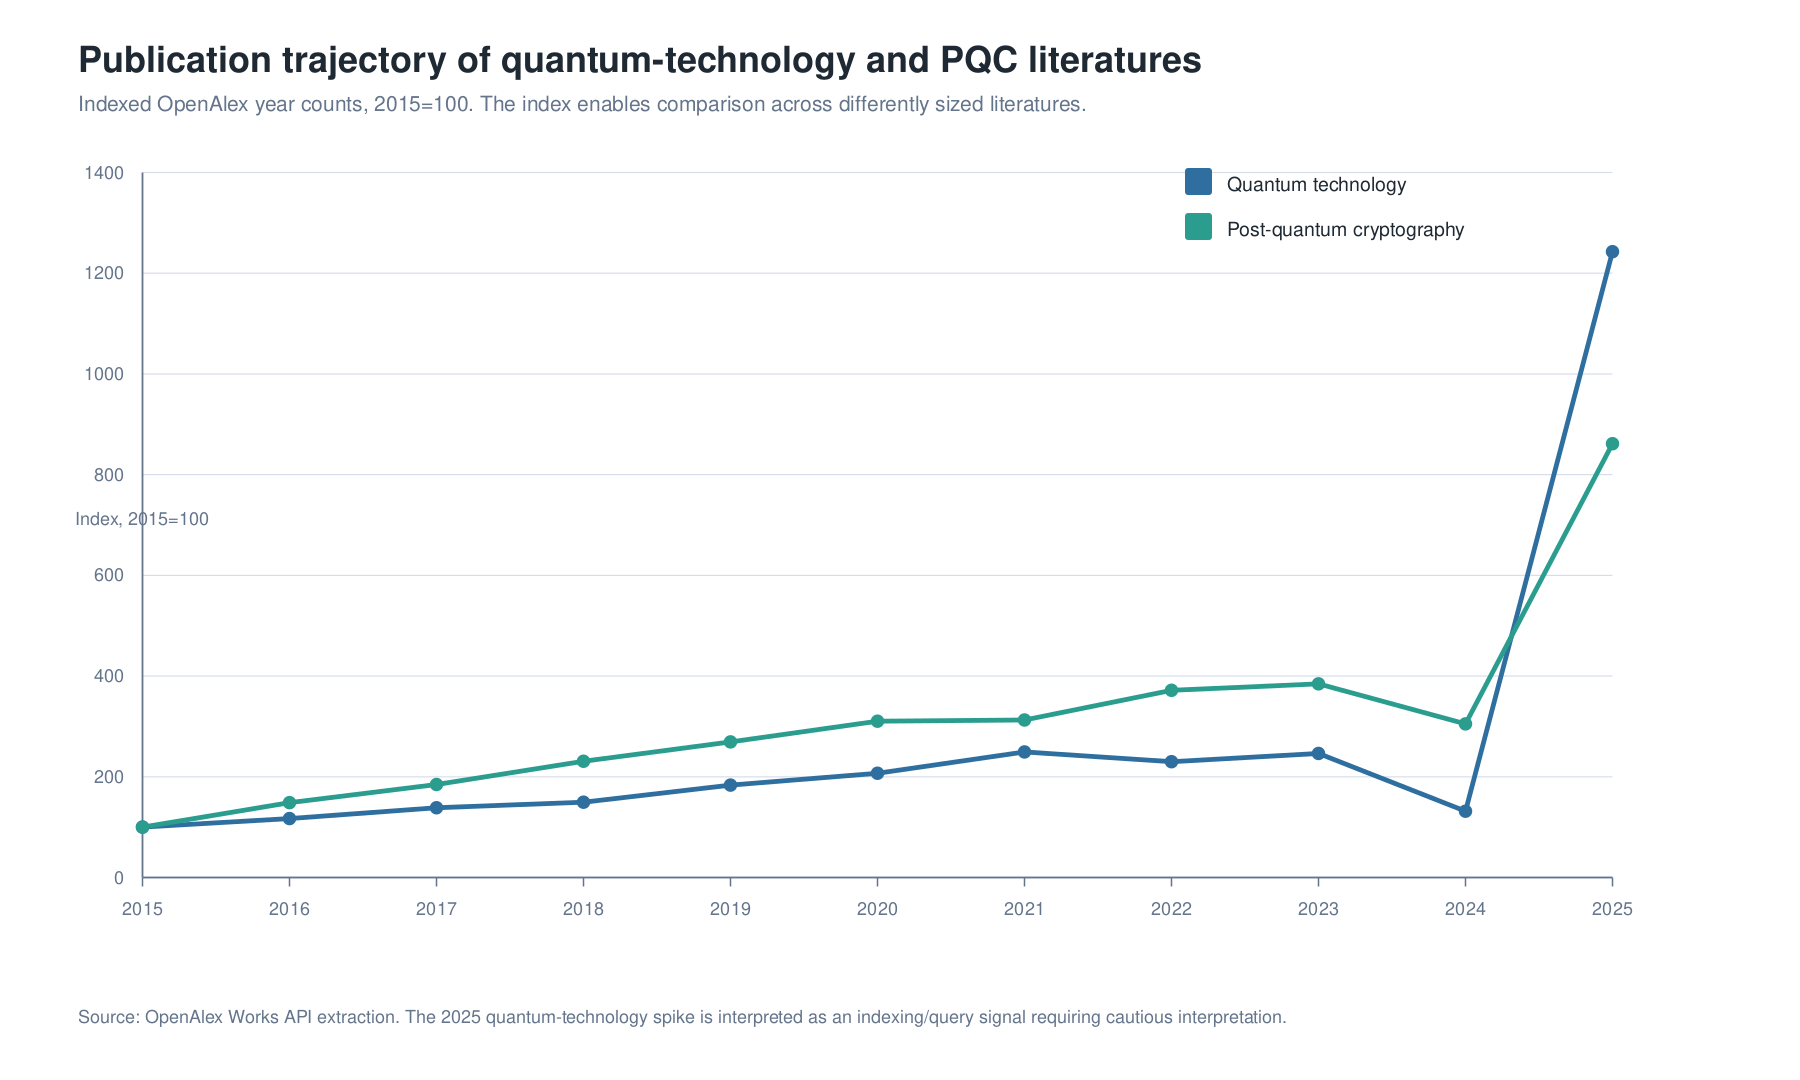
\includegraphics[width=0.95\textwidth,height=\textheight]{figures/fig2_publication_trends.png}
\caption{Trayectoria indexada de publicaciones en tecnología cuántica y
criptografía post-cuántica. Los conteos anuales de OpenAlex se indexan a
2015=100 para comparar literaturas de distinto tamaño. El salto de
tecnología cuántica en 2025 se interpreta como una señal de consulta e
indexación que requiere cautela.}
\end{figure}

\section{4. Evidencia cuantitativa: qué puede
medirse}\label{evidencia-cuantitativa-quuxe9-puede-medirse}

No existe una base pública integral que mida directamente la adopción
cuántica global. No hay un solo dataset que cubra sensores cuánticos
desplegados, enlaces QKD, migraciones PQC, pilotos empresariales, uso de
QCaaS, experimentos en la nube y flujos de trabajo de software cuántico.
Por ello, la evidencia se triangula mediante múltiples proxies.

\begin{longtable}[]{@{}
  >{\raggedright\arraybackslash}p{(\columnwidth - 4\tabcolsep) * \real{0.3333}}
  >{\raggedright\arraybackslash}p{(\columnwidth - 4\tabcolsep) * \real{0.3333}}
  >{\raggedright\arraybackslash}p{(\columnwidth - 4\tabcolsep) * \real{0.3333}}@{}}
\toprule\noalign{}
\begin{minipage}[b]{\linewidth}\raggedright
Capa de evidencia
\end{minipage} & \begin{minipage}[b]{\linewidth}\raggedright
Señal cuantitativa
\end{minipage} & \begin{minipage}[b]{\linewidth}\raggedright
Interpretación
\end{minipage} \\
\midrule\noalign{}
\endhead
\bottomrule\noalign{}
\endlastfoot
Compromisos públicos & La OCDE reporta aproximadamente USD 55.7 mil
millones en compromisos públicos cuánticos anunciados mundialmente desde
2013, a octubre de 2025 & Lo cuántico se ha vuelto una tecnología
estratégica de Estado \\
Apoyos públicos a I+D & Fundstat de la OCDE identifica USD 11.235 mil
millones PPP en 12,209 apoyos de I+D relacionados con tecnologías
cuánticas, 2015-2023 & La inversión pública se organiza mediante
programas de investigación y misión \\
Familias de patentes & El mapeo OCDE-OEP identifica 31,700 familias de
patentes cuánticas con primeros años de publicación entre 2005 y 2024;
el patentamiento cuántico se multiplicó por siete entre 2005 y 2024 y
creció alrededor de 20 por ciento CAGR desde 2014 & La invención se
acelera pero está geográficamente concentrada \\
Publicaciones & La consulta ``Quantum technology'' de OpenAlex devuelve
15,279 trabajos, 2015-2025; los países principales son Estados Unidos,
China, Alemania, Reino Unido y Francia & La capacidad científica de
absorción está distribuida de manera desigual \\
Publicaciones PQC & La consulta PQC de OpenAlex muestra a Estados
Unidos, India y China como afiliaciones líderes & La preparación PQC
depende de capacidades criptográficas y de software, no solo de hardware
físico \\
Preparación empresarial & La OCDE resume encuestas en las que la
expectativa de disrupción es alta, pero la planeación, los presupuestos
y la identificación de casos de uso son bajos & La conciencia no
equivale a preparación \\
Estándares & NIST finalizó ML-KEM, ML-DSA y SLH-DSA en 2024 & La
migración PQC ya es una agenda de implementación \\
\end{longtable}

El patrón más fuerte no es el crecimiento simple. Es la formación
desigual de capacidades. El financiamiento público aumenta, el
patentamiento se acelera y las publicaciones se concentran en un grupo
reducido de países. Al mismo tiempo, la preparación empresarial sigue
siendo débil. En la evidencia de preparación resumida por la OCDE, 97
por ciento de ejecutivos del Reino Unido en una encuesta esperaba
disrupción cuántica, pero solo alrededor de un tercio había iniciado
planeación; 87 por ciento de encuestados del sector financiero veía la
computación cuántica como oportunidad, mientras 73 por ciento carecía de
un caso de uso con ventaja comercial y 87 por ciento no tenía
presupuesto cuántico dedicado; evidencia de ISACA resumida por la OCDE
encontró que solo 20 por ciento de los encuestados tenía planes formales
de preparación cuántica pese a expectativas amplias de impacto
(\citeproc{ref-oecd2026}{OECD 2026}).

Esta es la brecha de adopción. Países y empresas están escuchando la
narrativa cuántica, pero muchos no han construido los mecanismos
requeridos para actuar sobre ella. La brecha no es un problema de
relaciones públicas. Es un problema de capacidades.

\begin{figure}
\centering
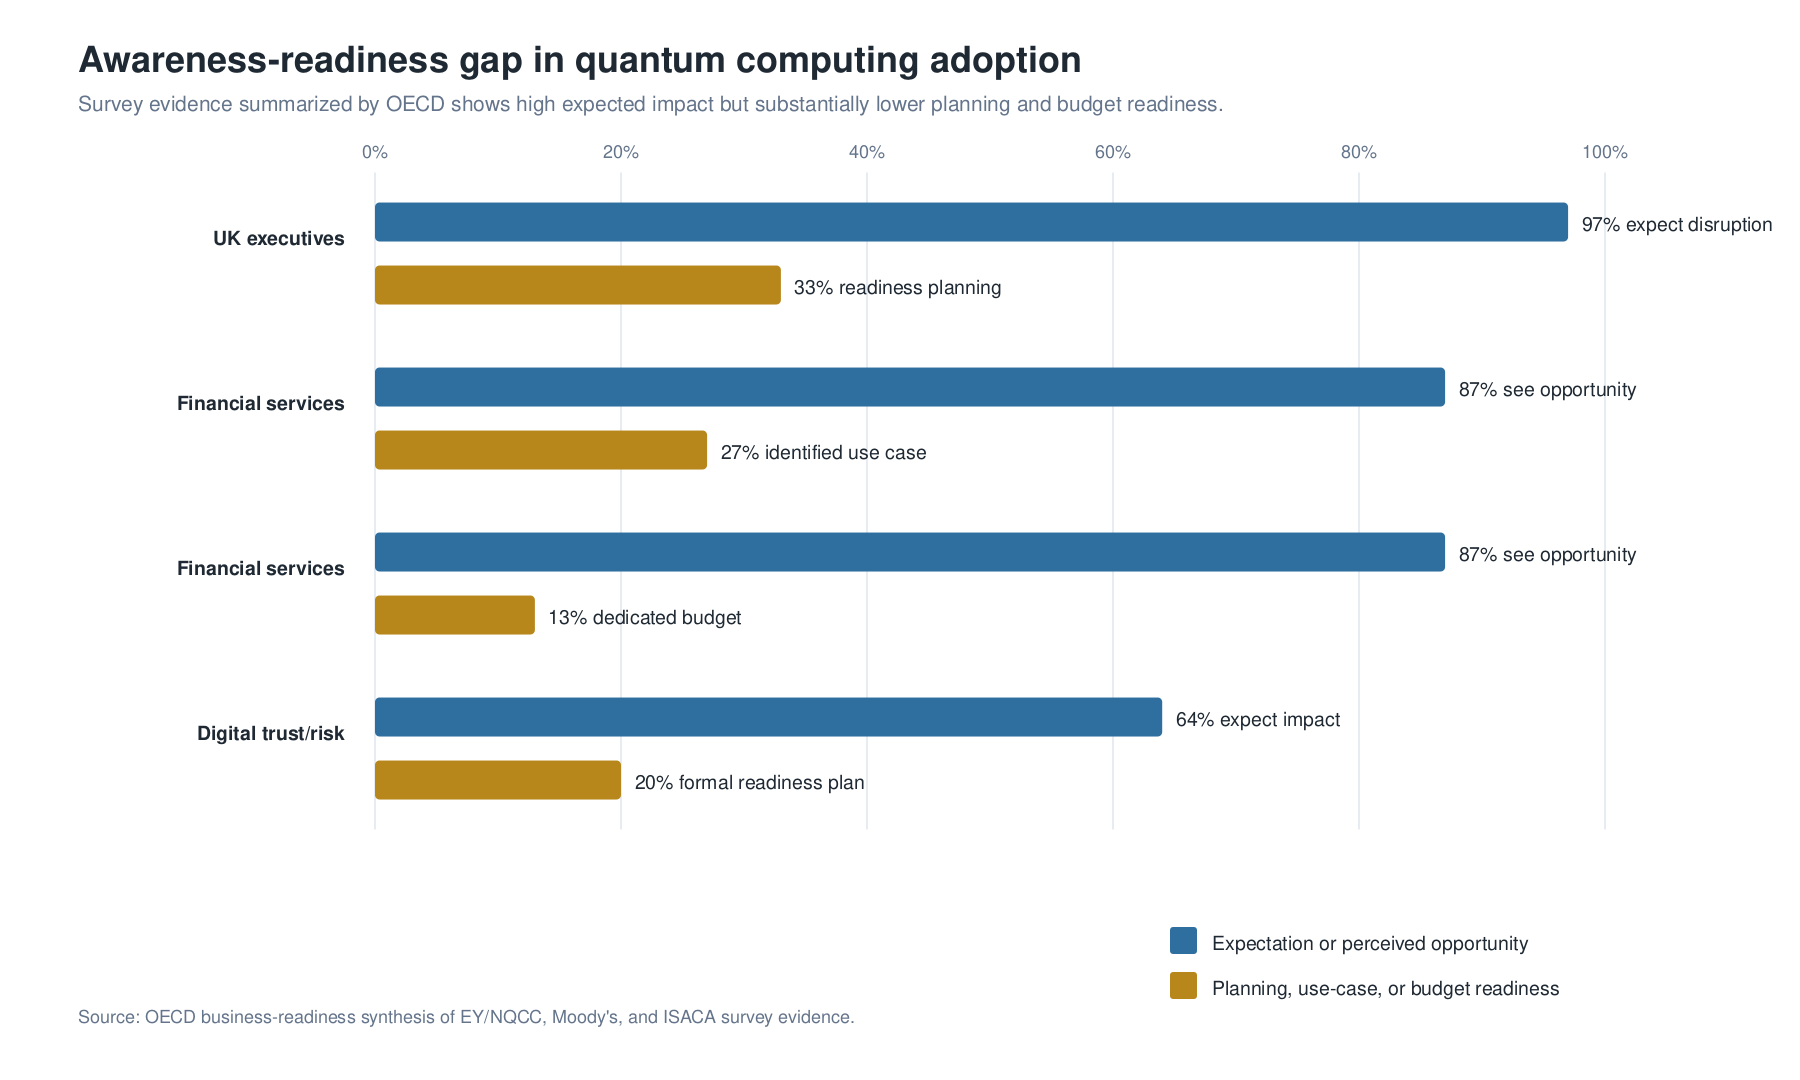
\includegraphics[width=0.95\textwidth,height=\textheight]{figures/fig3_readiness_gap.png}
\caption{Brecha entre conciencia y preparación en la adopción de
computación cuántica. La evidencia de encuestas resumida por la OCDE
indica que una alta expectativa de impacto coexiste con niveles mucho
menores de planeación, definición de casos de uso y formación de
presupuestos dedicados.}
\end{figure}

\section{5. Resultados: rutas de adopción por dominio
tecnológico}\label{resultados-rutas-de-adopciuxf3n-por-dominio-tecnoluxf3gico}

\subsection{5.1 Computación cuántica: alta opcionalidad, baja certeza de
corto
plazo}\label{computaciuxf3n-cuuxe1ntica-alta-opcionalidad-baja-certeza-de-corto-plazo}

La computación cuántica tiene el mayor potencial estratégico de largo
plazo y la mayor incertidumbre de adopción. Su fundamento teórico es
sólido. Los algoritmos cuánticos pueden ofrecer aceleraciones
asintóticas en clases específicas de problemas
(\citeproc{ref-montanaro2016}{Montanaro 2016}). La simulación cuántica y
la química son objetivos naturales porque las computadoras clásicas
enfrentan dificultades con la estructura exponencial de muchos sistemas
cuánticos (\citeproc{ref-georgescu2014}{Georgescu, Ashhab, y Nori 2014};
\citeproc{ref-cao2019}{Cao et~al. 2019}; \citeproc{ref-bauer2020}{Bauer
et~al. 2020}). Los algoritmos variacionales híbridos ofrecen rutas
experimentales de corto plazo (\citeproc{ref-peruzzo2014}{Peruzzo et~al.
2014}; \citeproc{ref-kandala2017}{Kandala et~al. 2017};
\citeproc{ref-cerezo2021}{Cerezo et~al. 2021};
\citeproc{ref-bharti2022}{Bharti et~al. 2022}).

La restricción dura es que las aplicaciones valiosas requieren circuitos
más profundos, menores tasas de error lógico y mejor verificación que
las disponibles en los dispositivos actuales. La tolerancia a fallas
sigue siendo el punto de transición entre dispositivos experimentales e
infraestructura confiable. Los códigos de superficie son una ruta líder
porque son compatibles con interacciones locales bidimensionales, pero
imponen grandes sobrecostos (\citeproc{ref-fowler2012}{Fowler et~al.
2012}; \citeproc{ref-campbell2017}{Campbell, Terhal, y Vuillot 2017}).
Las estimaciones de recursos para máquinas criptográficamente relevantes
siguen siendo altas, aun cuando mejores algoritmos reducen
requerimientos (\citeproc{ref-gidney2021}{Gidney y Ekera 2021}).

La implicación para adopción es que la computación cuántica funciona en
el corto plazo como un dominio de aprendizaje, evaluación comparativa y
valor de opción. Las acciones nacionales y empresariales más racionales
no son el despliegue masivo, sino la experimentación dirigida, la
formación de talento, la evaluación algorítmica, el acceso a plataformas
QCaaS y la comparación cuidadosa con alternativas clásicas.

\subsection{5.2 Sensórica cuántica: el dominio de valor público más
inmediato}\label{sensuxf3rica-cuuxe1ntica-el-dominio-de-valor-puxfablico-muxe1s-inmediato}

La sensórica cuántica es el dominio de aplicación de corto plazo más
fuerte porque puede producir valor sin computadoras cuánticas
universales tolerantes a fallas. Usa sistemas cuánticos como
dispositivos de medición: relojes atómicos para tiempo, magnetómetros
para campos magnéticos, gravímetros para mapeo del subsuelo, sensores
inerciales para navegación y defectos cuánticos en diamante para
sensórica magnética local (\citeproc{ref-degen2017}{Degen, Reinhard, y
Cappellaro 2017}; \citeproc{ref-barry2016}{Barry et~al. 2016}). La
propuesta de valor no es ``cómputo más rápido'', sino mejor información
sobre el mundo físico.

La distinción es importante para la política pública. Muchos países
tienen problemas urgentes en agua, infraestructura, minería, salud,
energía, navegación, monitoreo fronterizo, riesgo sísmico, vigilancia
ambiental y control de calidad industrial. La sensórica cuántica puede
vincularse a estas misiones antes de que la computación cuántica pueda
vincularse a una transformación empresarial general. La barrera no es la
incertidumbre teórica, sino el despliegue en campo: los instrumentos
requieren robustez, calibración, costo-efectividad, interoperabilidad y
relevancia operativa.

\subsection{5.3 Comunicación cuántica: estratégica, especializada e
intensiva en
infraestructura}\label{comunicaciuxf3n-cuuxe1ntica-estratuxe9gica-especializada-e-intensiva-en-infraestructura}

La comunicación cuántica tiene fuerte relevancia estratégica de largo
plazo, especialmente para distribución de entrelazamiento, enlaces
seguros, sensórica distribuida y redes cuánticas futuras
(\citeproc{ref-kimble2008}{Kimble 2008};
\citeproc{ref-wehner2018}{Wehner, Elkouss, y Hanson 2018}). QKD ya ha
avanzado más allá de la demostración puramente de laboratorio, y la
literatura de seguridad se ha vuelto sofisticada respecto a dispositivos
realistas, canales laterales y protocolos independientes del dispositivo
de medición (\citeproc{ref-pirandola2020}{Pirandola et~al. 2020};
\citeproc{ref-xu2020}{Xu et~al. 2020}).

La crítica es igualmente importante. QKD no elimina la necesidad de
autenticación, seguridad de endpoints, ingeniería de redes, estándares
de adquisición ni análisis costo-beneficio. Requiere infraestructura
especializada y puede estar limitada por pérdida, distancia, supuestos
de nodos confiables y aseguramiento de dispositivos. Los repetidores
cuánticos son el análogo de red de la tolerancia a fallas: sin
repetidores, memorias, intercambio de entrelazamiento e interfaces de
baja pérdida confiables, las redes cuánticas de gran escala siguen
restringidas.

En consecuencia, la comunicación cuántica se persigue mejor mediante
testbeds dirigidos y enlaces de alto valor, no mediante afirmaciones
amplias de que reemplazará la ciberseguridad existente. Su valor
nacional reside en aprendizaje estratégico, experimentación telecom,
nichos de alta seguridad y preparación para futuras redes cuánticas.

\subsection{5.4 Criptografía post-cuántica: el primer mandato nacional
de
adopción}\label{criptografuxeda-post-cuuxe1ntica-el-primer-mandato-nacional-de-adopciuxf3n}

La PQC es el dominio de adopción más urgente porque aborda una
transición real de seguridad que puede comenzar antes de que existan
computadoras cuánticas criptográficamente relevantes. El algoritmo de
Shor amenaza RSA, Diffie-Hellman y criptografía de curva elíptica una
vez que existan máquinas tolerantes a fallas de gran escala. El riesgo
relevante no es solo un ataque futuro; es la recolección actual de datos
cifrados de larga vida (\citeproc{ref-mosca2018}{Mosca 2018}). Los
estándares de NIST de 2024 ofrecen a las organizaciones un objetivo
concreto de migración, especialmente ML-KEM, ML-DSA y SLH-DSA
(\citeproc{ref-nist2024}{NIST 2024}).

La parte difícil no es elegir un algoritmo en aislamiento. La migración
requiere inventarios criptográficos, cripto-agilidad, coordinación con
proveedores, pruebas de protocolos, reemplazo de sistemas heredados,
lenguaje de adquisición, gobernanza de cumplimiento y priorización por
vida útil de los datos. La PQC es, por tanto, un programa de
infraestructura digital. Tratarla como un parche estrecho de
ciberseguridad subestima el trabajo institucional implicado.

\section{6. Comparación de hardware y economía de qubits
lógicos}\label{comparaciuxf3n-de-hardware-y-economuxeda-de-qubits-luxf3gicos}

Ninguna modalidad de hardware ha ganado. Cada plataforma expresa un
compromiso de ingeniería distinto.

\begin{longtable}[]{@{}
  >{\raggedright\arraybackslash}p{(\columnwidth - 6\tabcolsep) * \real{0.2500}}
  >{\raggedright\arraybackslash}p{(\columnwidth - 6\tabcolsep) * \real{0.2500}}
  >{\raggedright\arraybackslash}p{(\columnwidth - 6\tabcolsep) * \real{0.2500}}
  >{\raggedright\arraybackslash}p{(\columnwidth - 6\tabcolsep) * \real{0.2500}}@{}}
\toprule\noalign{}
\begin{minipage}[b]{\linewidth}\raggedright
Modalidad
\end{minipage} & \begin{minipage}[b]{\linewidth}\raggedright
Fortaleza
\end{minipage} & \begin{minipage}[b]{\linewidth}\raggedright
Cuello de botella
\end{minipage} & \begin{minipage}[b]{\linewidth}\raggedright
Interpretación estratégica
\end{minipage} \\
\midrule\noalign{}
\endhead
\bottomrule\noalign{}
\endlastfoot
Qubits superconductores & Compuertas rápidas, ecosistema industrial
fuerte, ruta de microfabricación, disponibilidad en nube & Cableado
criogénico, pérdida dieléctrica, crosstalk, carga térmica, calibración &
Plataforma fuerte de corto plazo, pero la escala depende de la economía
de control y corrección de errores \\
Iones atrapados & Alta fidelidad, larga coherencia, uniformidad natural
de qubits, conectividad flexible & Velocidad de compuertas, transporte,
calentamiento, complejidad láser/control & Calidad excelente, pero la
escala de ingeniería y el throughput siguen siendo preguntas
centrales \\
Átomos neutros & Arreglos grandes, geometría reconfigurable,
escalabilidad prometedora & Pérdida de átomos, leakage, fidelidad de
compuertas, lectura, control óptico & Opción fuerte para simulación y
escalamiento, con preguntas abiertas sobre arquitectura tolerante a
fallas \\
Fotónica & Medio natural de comunicación, potencial a temperatura
ambiente, compatibilidad con redes & Pérdida de fotones, compuertas
deterministas, integración de fuentes y detectores & Estratégicamente
importante para redes y algunas arquitecturas de cómputo \\
Recocido cuántico & Sistemas disponibles y experimentos de optimización
& Universalidad limitada, ambigüedad de benchmarks, sobrecosto de mapeo
& Útil para experimentación cuando se compara contra heurísticas
clásicas \\
\end{longtable}

Las plataformas superconductoras han avanzado rápidamente y son
revisadas en detalle por Krantz et~al. (\citeproc{ref-krantz2019}{2019})
y Kjaergaard et~al. (\citeproc{ref-kjaergaard2020}{2020}). Los sistemas
de iones atrapados son revisados por Bruzewicz et~al.
(\citeproc{ref-bruzewicz2019}{2019}). Los sistemas de átomos neutros son
revisados por Saffman (\citeproc{ref-saffman2016}{2016}) y Henriet
et~al. (\citeproc{ref-henriet2020}{2020}). Los sistemas fotónicos son
revisados por Slussarenko y Pryde
(\citeproc{ref-slussarenko2019}{2019}). La comparación muestra por qué
el conteo de qubits es una métrica débil. Un dispositivo con más qubits
físicos puede ser menos valioso que uno más pequeño con mejor fidelidad
de compuertas, menor ruido correlacionado, mejor conectividad o una ruta
más clara hacia la supresión de error lógico.

La métrica estratégica es la economía de qubits lógicos. Una computadora
cuántica útil no se definirá por el número de qubits físicos que
contenga. Se definirá por el costo, la confiabilidad y la velocidad de
sus operaciones lógicas. Las métricas relevantes incluyen tasa de error
lógico, distancia de código, tiempo de ciclo, latencia de
decodificación, leakage, conectividad, estabilidad de calibración,
profundidad de circuito con fidelidad útil, costo energético y recursos
físicos por qubit lógico. Proctor et~al.
(\citeproc{ref-proctor2022}{2022}) sostienen que la capacidad de una
computadora cuántica se mide por los programas que un procesador puede
ejecutar con éxito, no por un benchmark escalar único. Ese es el
estándar requerido para política pública y adquisición.

\section{7. Dominios de aplicación: promesa, evidencia y
crítica}\label{dominios-de-aplicaciuxf3n-promesa-evidencia-y-cruxedtica}

\subsection{7.1 Química y materiales}\label{quuxedmica-y-materiales}

La química y la ciencia de materiales siguen siendo el caso de
aplicación más fuerte de largo plazo. Las computadoras cuánticas podrían
eventualmente simular sistemas moleculares y de materiales de forma más
natural que las máquinas clásicas
(\citeproc{ref-georgescu2014}{Georgescu, Ashhab, y Nori 2014};
\citeproc{ref-cao2019}{Cao et~al. 2019}; \citeproc{ref-bauer2020}{Bauer
et~al. 2020}). Las aplicaciones potenciales incluyen catalizadores,
baterías, fármacos, superconductores de alta temperatura, corrosión,
fertilizantes, polímeros, semiconductores y captura de carbono.

La crítica es que la relevancia científica no produce adopción
industrial automáticamente. Un flujo de trabajo útil mejora una decisión
en descubrimiento de fármacos, diseño de materiales o manufactura.
Produce precisión relevante, se integra con experimentos de laboratorio
y reduce tiempo o costo. La ruta de adopción es por tanto híbrida:
algoritmos cuánticos, cómputo clásico de alto desempeño, modelos de IA,
experimentos y expertos de dominio trabajando juntos.

\subsection{7.2 Optimización}\label{optimizaciuxf3n}

La optimización se cita con frecuencia como la oportunidad comercial más
temprana, pero también es el área más fácil de exagerar. Logística,
optimización de portafolios, calendarización, gestión de redes
eléctricas y cadenas de suministro son valiosas, pero la optimización
clásica es extraordinariamente fuerte. Programación entera mixta,
programación por restricciones, heurísticas, algoritmos de aproximación,
GPUs y solvers específicos de dominio ya funcionan bien. Una afirmación
de optimización cuántica solo es creíble cuando supera el mejor baseline
clásico en una instancia relevante a un costo relevante.

El rol más realista de corto plazo es exploratorio: recocido cuántico,
flujos tipo QAOA y métodos inspirados en lo cuántico pueden ayudar a
identificar clases de problemas y prácticas de software. No son
reemplazos generales para la investigación de operaciones.

\subsection{7.3 Finanzas}\label{finanzas}

Las finanzas son atractivas porque pequeñas mejoras en riesgo,
optimización, muestreo o precios pueden crear gran valor. Orus, Mugel, y
Lizaso (\citeproc{ref-orus2019}{2019}) y Egger et~al.
(\citeproc{ref-egger2020}{2020}) revisan aplicaciones potenciales,
incluyendo optimización de portafolios, aceleración de Monte Carlo,
análisis de riesgo, calificación crediticia y valuación de derivados.
Las instituciones serias no preguntarán si la computación cuántica está
de moda. Preguntarán si mejora calidad de modelo, velocidad,
auditabilidad regulatoria y asignación de capital frente a métodos
clásicos.

\subsection{7.4 Aprendizaje automático e
IA}\label{aprendizaje-automuxe1tico-e-ia}

El aprendizaje automático cuántico es intelectualmente rico, pero
comercialmente inmaduro. Biamonte et~al.
(\citeproc{ref-biamonte2017}{2017}) identifican razones por las que los
sistemas cuánticos podrían soportar modelos útiles de aprendizaje.
Schuld y Killoran (\citeproc{ref-schuld2019}{2019}) conectan mapas de
características cuánticas con métodos kernel. McClean et~al.
(\citeproc{ref-mcclean2018}{2018}) muestran que el entrenamiento puede
fallar por mesetas estériles. La recomendación de política es directa:
QML pertenece al portafolio de investigación, no a afirmaciones
exageradas de transformación empresarial. El valor de corto plazo puede
venir más de la IA mejorando sistemas cuánticos -calibración, mitigación
de errores, diseño de pulsos, descubrimiento de materiales y control-
que de sistemas cuánticos mejorando la IA convencional.

\subsection{7.5 Ciberseguridad}\label{ciberseguridad}

La ciberseguridad es la aplicación transversal más inmediata porque la
migración PQC afecta casi todo sistema digital. El asunto central de
política es el tiempo. Datos que requieren confidencialidad por 10, 20 o
30 años pueden ser vulnerables al descifrado cuántico futuro. Grandes
organizaciones pueden requerir muchos años para inventariar y migrar
activos criptográficos. Si la suma de vida útil del dato y tiempo de
migración excede el tiempo hasta una computadora cuántica
criptográficamente relevante, la acción ya llega tarde por definición
(\citeproc{ref-mosca2018}{Mosca 2018}).

\section{8. Cómputo de alto desempeño y computación
cuántica}\label{cuxf3mputo-de-alto-desempeuxf1o-y-computaciuxf3n-cuuxe1ntica}

La ruta de adopción de la computación cuántica es inseparable del
cómputo de alto desempeño. Es improbable que las computadoras cuánticas
reemplacen a las supercomputadoras clásicas como máquinas de propósito
general. La transición más plausible es un modelo de aceleradores en el
cual las unidades de procesamiento cuántico se integran a entornos HPC
heterogéneos junto con CPUs, GPUs, almacenamiento, gestores de flujos de
trabajo, calendarizadores y pilas de software científico. En esta
arquitectura, la computación cuántica se invoca solo para subrutinas
donde una representación cuántica podría mejorar simulación, muestreo,
optimización o tareas de álgebra lineal, mientras el HPC clásico realiza
preparación de datos, orquestación, mitigación de errores, ciclos de
optimización, verificación y post-procesamiento.

La investigación reciente en HPC-QC refleja esta transición. Cranganore
et~al. (\citeproc{ref-cranganore2024}{2024}) formalizan flujos de
trabajo científicos híbridos cuántico-clásicos e identifican requisitos
de gestión de flujos para mapear pipelines científicos clásicos hacia
recursos híbridos. Beck et~al. (\citeproc{ref-beck2024}{2024}) enmarcan
la computación cuántica como acelerador computacional dentro de
ecosistemas científicos HPC, enfatizando integración independiente del
hardware, benchmarks, interfaces de usuario y gestión de workflows. Liu
et~al. (\citeproc{ref-liu2024}{2024}) desarrollan una perspectiva HPC
centrada en lo cuántico para química cuántica, donde algoritmos
cuánticos, emuladores cuánticos y recursos HPC clásicos apoyan
conjuntamente la simulación química. Esta literatura desplaza la
pregunta de ``¿cuándo reemplazarán las computadoras cuánticas a las
supercomputadoras?'' hacia ``¿qué componentes de un flujo científico
pueden delegarse a una QPU bajo restricciones realistas de latencia,
ruido, colas y verificación?''

La visión HPC modifica cuatro elementos de la estrategia cuántica.
Primero, modifica la infraestructura. Un ecosistema útil de computación
cuántica requiere no solo QPUs y cuentas en la nube, sino también
calendarizadores, middleware, compiladores, software de mitigación de
errores, protocolos de movimiento de datos, sistemas de procedencia,
controles de reproducibilidad e interfaces con códigos científicos
existentes. Segundo, modifica la evaluación comparativa. Una subrutina
cuántica debe evaluarse dentro de un flujo completo, incluyendo costo de
carga de datos, tiempo de optimización clásica, latencia de cola,
sobrecosto de mitigación de errores y validación contra baselines HPC
clásicos. Tercero, modifica la formación laboral. La adopción de
computación cuántica requiere científicos computacionales e ingenieros
HPC capaces de descomponer aplicaciones en componentes clásicos y
cuánticos, no solo físicos que entienden qubits. Cuarto, modifica la
adquisición nacional. Un país que invierte en computación cuántica sin
capacidad de integración HPC corre el riesgo de comprar dispositivos
aislados incapaces de sostener flujos científicos o industriales.

La complementariedad es especialmente importante para economías
cuánticas emergentes y de ingreso medio. La propiedad doméstica de una
computadora cuántica líder puede ser irrealista en el corto plazo, pero
el acceso a centros HPC, clusters GPU, sistemas de workflow científico y
QPUs en la nube puede construir capacidad de absorción significativa. El
objetivo estratégico no es una transición binaria de HPC a computación
cuántica. Es la construcción de un continuo HPC-QC en el que la
supercomputación clásica permanece como sustrato operativo y la
computación cuántica entra como acelerador especializado cuando la
evidencia lo justifica.

\section{9. Estrategia nacional
comparada}\label{estrategia-nacional-comparada}

Los modelos nacionales revelan teorías estratégicas distintas.

Estados Unidos combina coordinación federal, laboratorios nacionales,
universidades, capital de riesgo, grandes plataformas en la nube e
investigación vinculada a defensa. Su ventaja es la diversidad
ecosistémica y la profundidad del capital privado. Su debilidad es la
fragmentación y la traducción desigual entre agencias y sectores.

China ha enfatizado inversión dirigida por el Estado, infraestructura de
comunicación segura y autosuficiencia tecnológica. Su ventaja es la
coordinación y el foco estratégico. Su debilidad puede ser menor
transparencia y riesgo de sobredimensionar infraestructura simbólica
antes de que exista valor operativo claro.

Europa enfatiza coordinación transfronteriza, redes públicas de
investigación, estándares y autonomía estratégica. Su ventaja es la
coordinación institucional y la calidad de investigación. Su debilidad
es la velocidad de comercialización y la fragmentación entre mercados
nacionales.

Los países de ingreso medio e intensivos en manufactura enfrentan un
problema distinto. No pueden simplemente copiar los programas más
grandes. Su oportunidad estratégica es la construcción selectiva de
capacidades: migración PQC, sensórica cuántica para misiones públicas,
acceso a computación cuántica mediado por la nube, laboratorios de
metrología, redes de fuerza laboral y participación en estándares. La
meta correcta no es poseer de inmediato cada capa del stack. Es evitar
convertirse solo en comprador de tecnologías cuánticas diseñadas,
evaluadas y gobernadas en otra parte.

\section{10. Hacia un modelo nacional de capacidades
cuánticas}\label{hacia-un-modelo-nacional-de-capacidades-cuuxe1nticas}

La evidencia apoya un modelo de capacidades con siete pilares.

\begin{longtable}[]{@{}
  >{\raggedright\arraybackslash}p{(\columnwidth - 4\tabcolsep) * \real{0.3333}}
  >{\raggedright\arraybackslash}p{(\columnwidth - 4\tabcolsep) * \real{0.3333}}
  >{\raggedright\arraybackslash}p{(\columnwidth - 4\tabcolsep) * \real{0.3333}}@{}}
\toprule\noalign{}
\begin{minipage}[b]{\linewidth}\raggedright
Pilar
\end{minipage} & \begin{minipage}[b]{\linewidth}\raggedright
Capacidad central
\end{minipage} & \begin{minipage}[b]{\linewidth}\raggedright
Pregunta institucional principal
\end{minipage} \\
\midrule\noalign{}
\endhead
\bottomrule\noalign{}
\endlastfoot
Frontera científica & Investigación en información cuántica, algoritmos,
metrología, materiales, corrección de errores, fundamentos & ¿Puede el
país participar en la producción de conocimiento de frontera? \\
Transición de seguridad & Migración PQC, cripto-agilidad, protección de
datos de larga vida & ¿Pueden los sistemas críticos mantenerse seguros
durante la transición cuántica? \\
Sensórica y metrología & Relojes atómicos, magnetometría, gravimetría,
sensórica inercial, calibración & ¿Puede la medición cuántica resolver
problemas nacionales en territorio, agua, salud, energía e
infraestructura? \\
Acceso computacional HPC-QC & QCaaS, integración HPC, flujos híbridos,
benchmarks, software cuántico & ¿Pueden las instituciones aprender sin
encierro prematuro en hardware y preservando continuidad con
infraestructura científica de cómputo? \\
Estándares y adquisición & Benchmarking, interoperabilidad, evaluación
de proveedores, criterios anti-hype & ¿Pueden compradores públicos y
privados distinguir desempeño de narrativa? \\
Fuerza laboral & Investigadores, ingenieros, técnicos, profesionales de
ciberseguridad, responsables de compras & ¿Puede el ecosistema construir
el eslabón intermedio entre doctorados en física y despliegue
operativo? \\
Posición industrial & Componentes, sistemas de control, fotónica,
criogenia, software, integración de sensores & ¿Dónde pueden entrar
realistamente las empresas nacionales en la cadena de valor? \\
\end{longtable}

El pilar de fuerza laboral merece énfasis. Kaur y Venegas-Gomez
(\citeproc{ref-kaur2022}{2022}) muestran que las iniciativas globales de
educación cuántica se expanden, pero el problema laboral no consiste
solo en más doctorados. Las industrias cuánticas requieren técnicos e
ingenieros capaces de alinear láseres, operar criostatos, construir
sistemas de control RF, manejar vacío, escribir firmware, calibrar,
diseñar interfaces de software, auditar criptografía y traducir
problemas de dominio en flujos de trabajo verificables. Una nación que
forma solo investigadores, pero no operadores, seguirá dependiendo de
sistemas importados.

\begin{figure}
\centering
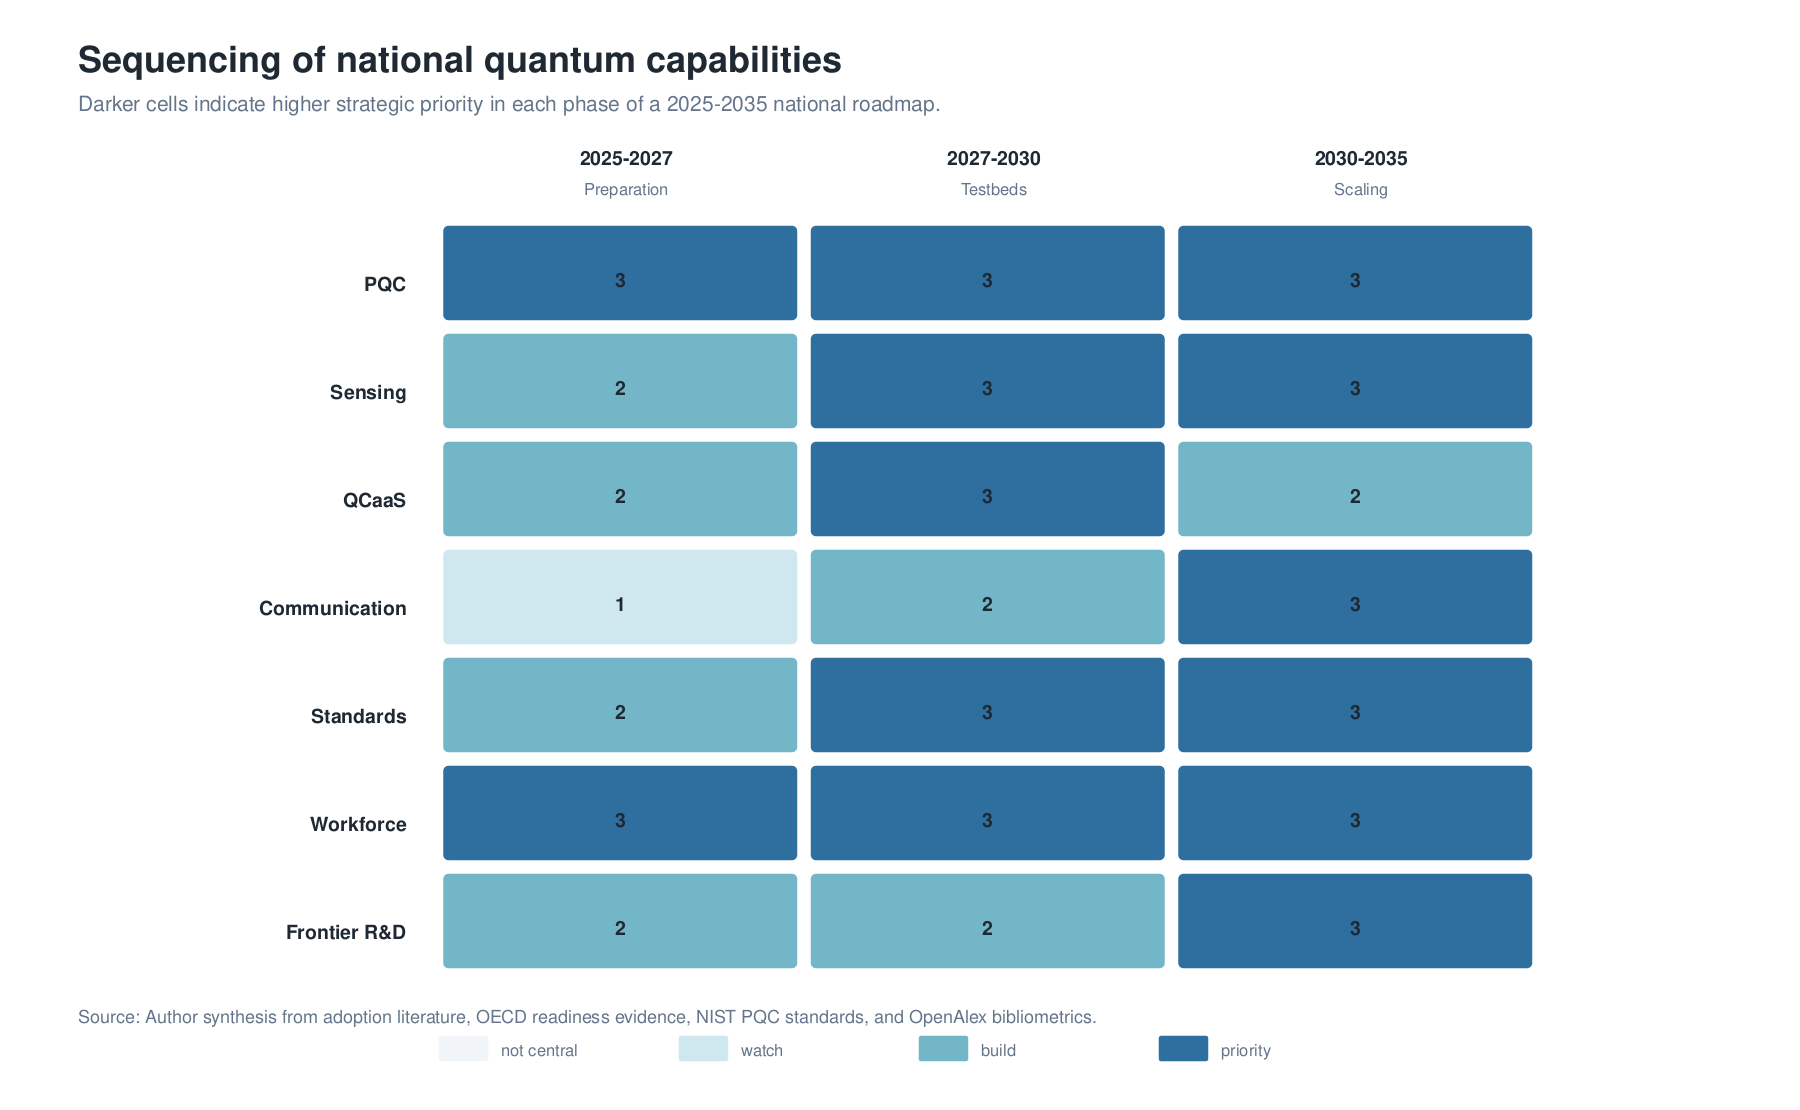
\includegraphics[width=0.95\textwidth,height=\textheight]{figures/fig4_capability_heatmap.png}
\caption{Secuenciación de capacidades cuánticas nacionales. El mapa de
calor puntúa la prioridad estratégica en tres fases de hoja de ruta y
enfatiza que PQC, fuerza laboral, estándares, sensórica, QCaaS,
comunicación e I+D de frontera maduran en horizontes de política
distintos.}
\end{figure}

\section{11. Hoja de ruta estratégica,
2025-2035}\label{hoja-de-ruta-estratuxe9gica-2025-2035}

\subsection{11.1 Fase I: preparación y seguridad,
2025-2027}\label{fase-i-preparaciuxf3n-y-seguridad-2025-2027}

La primera fase no consiste en comprar una computadora cuántica
nacional. Consiste en convertirse en un adoptante competente. Las
acciones institucionales centrales incluyen una oficina de preparación
cuántica, inventarios de activos criptográficos, prioridades de
migración PQC para datos de larga vida, lenguaje de adquisición para
sistemas cuánticamente seguros, estudios de factibilidad de sensórica
cuántica, acceso QCaaS para universidades y agencias, entrenamiento en
flujos HPC-QC y módulos de fuerza laboral para ingenieros, profesionales
de ciberseguridad y tomadores de decisión del sector público.

Los productos medibles no son comunicados de prensa. Son inventarios,
personal capacitado, pipelines de casos de uso, requisitos verificables,
estándares de adquisición y competencia institucional básica.

\subsection{11.2 Fase II: testbeds y pilotos de misión,
2027-2030}\label{fase-ii-testbeds-y-pilotos-de-misiuxf3n-2027-2030}

La segunda fase se centra en aprendizaje operativo. Los pilotos de
sensórica cuántica pueden vincularse a agua, energía, salud, geodesia,
infraestructura, minería y riesgo ambiental. La migración PQC pasa de
planeación a implementación por etapas. Los testbeds de software
cuántico evalúan algoritmos contra baselines clásicos. Los centros HPC
prueban flujos híbridos cuántico-clásicos, incluyendo integración de
calendarizadores, transición de simulador a hardware y procedencia de
workflows. Instituciones de telecomunicaciones e investigación pueden
probar QKD y componentes tempranos de red donde los enlaces de alto
valor justifiquen el costo. Los laboratorios de estándares evalúan
afirmaciones de proveedores.

El riesgo principal en esta fase es el \emph{quantum washing}.
Proveedores y agencias pueden etiquetar sistemas clásicos, inspirados en
lo cuántico o inmaduros como avances estratégicos. La protección es
disciplina de benchmarks: cada piloto requiere un baseline clásico, una
métrica de desempeño, una métrica de costo, un método de verificación y
una regla de decisión.

\subsection{11.3 Fase III: escalamiento selectivo e integración de
frontera,
2030-2035}\label{fase-iii-escalamiento-selectivo-e-integraciuxf3n-de-frontera-2030-2035}

La tercera fase escala solo aquello que ha demostrado valor. Los
sistemas de sensórica que resuelvan problemas de misión pueden pasar a
adquisición. La PQC puede convertirse en estándar en toda la
infraestructura digital pública. La computación cuántica puede
expandirse donde los workflows muestren ventaja creíble o donde el valor
científico y de formación justifique continuar la experimentación. La
investigación nacional profundiza en corrección de errores, qubits
lógicos, repetidores cuánticos, seguridad independiente de dispositivos,
metrología cuántica, materiales cuánticos y fundamentos.

\begin{figure}
\centering
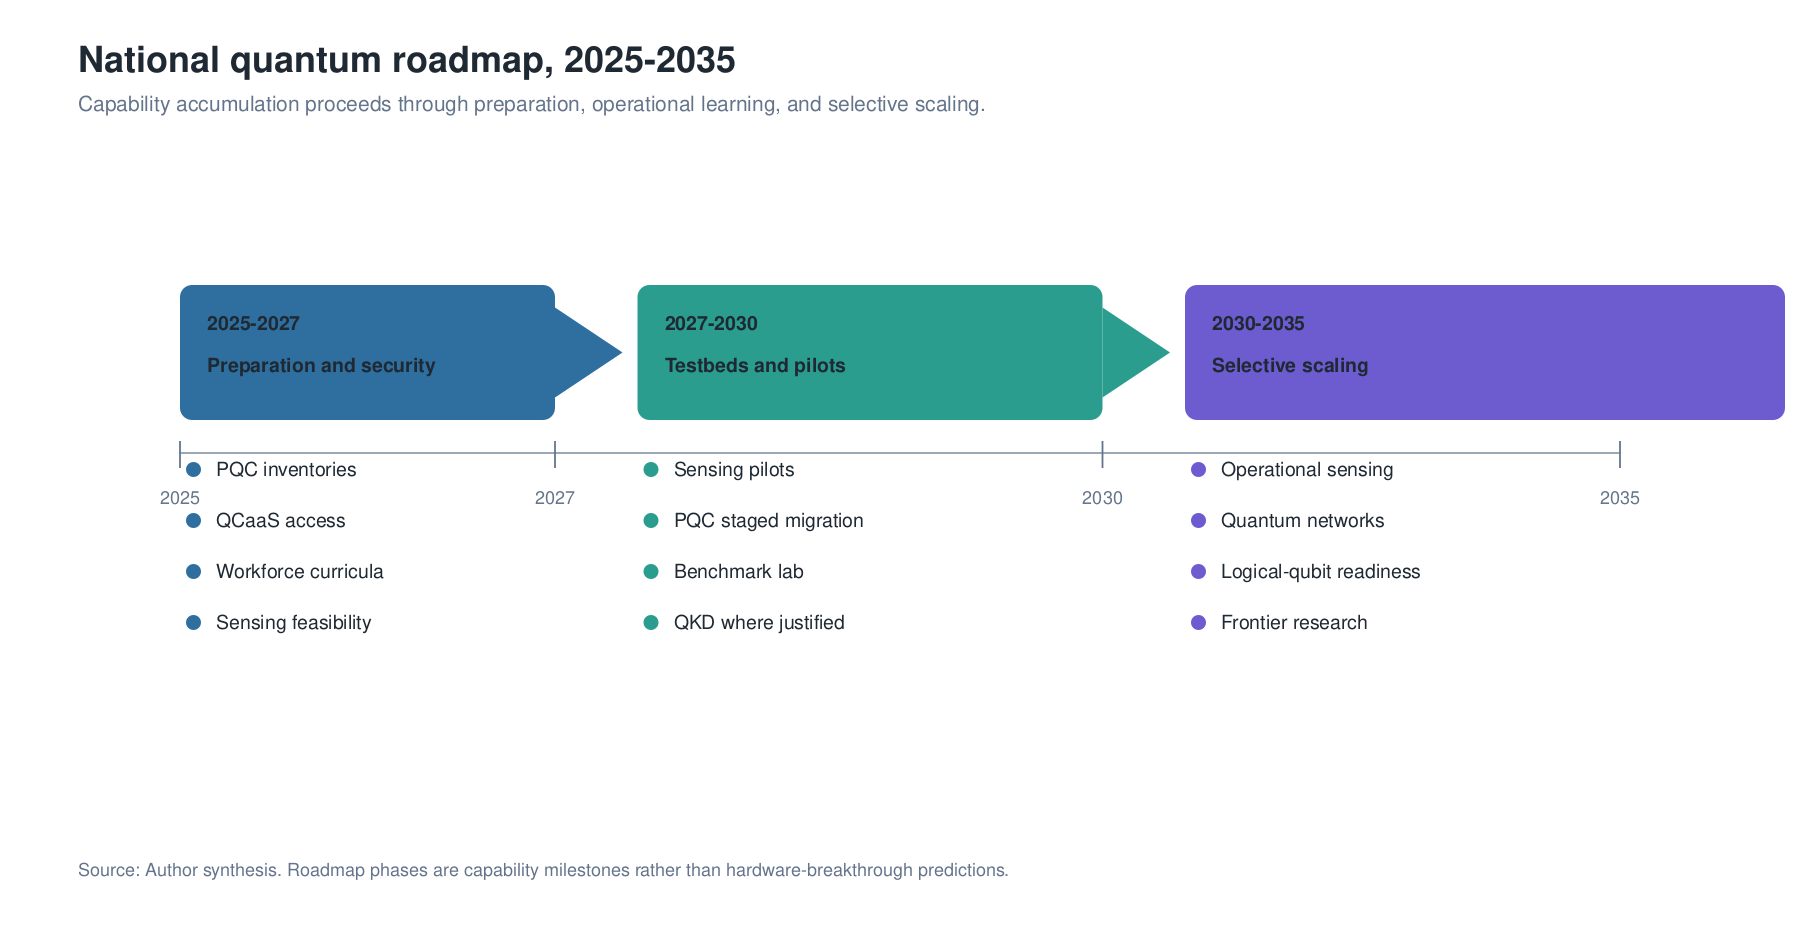
\includegraphics[width=0.95\textwidth,height=\textheight]{figures/fig5_roadmap_timeline.png}
\caption{Hoja de ruta para la formación de capacidades cuánticas
nacionales, 2025-2035. La secuencia se organiza alrededor de preparación
institucional, aprendizaje operativo y escalamiento selectivo, no de la
predicción de un solo avance de hardware.}
\end{figure}

El objetivo estratégico es la opcionalidad. Para 2035, la nación exitosa
no es necesariamente la que anuncia la computadora cuántica más grande.
Es la que cuenta con personas formadas, criptografía segura, testbeds
funcionales, capacidad de estándares, capacidad metrológica, pilotos de
dominio, alianzas internacionales y una base de investigación conectada
con la frontera.

\section{12. Agenda de investigación de
frontera}\label{agenda-de-investigaciuxf3n-de-frontera}

La estrategia nacional cuántica incluye temas de frontera que no son
inmediatamente comerciales. Estas áreas generan instrumentos, expertise
y autonomía de largo plazo.

\textbf{Economía de qubits lógicos.} La investigación se desplaza de
conteos de qubits físicos al costo de operaciones lógicas. Esto incluye
corrección de errores, decodificadores, gestión de leakage, sobrecosto
de estados mágicos, códigos qLDPC y estimaciones de recursos específicas
por arquitectura.

\textbf{Punto de equilibrio de redes cuánticas.} Repetidores, memorias,
transductores e intercambio de entrelazamiento son el equivalente de red
de la tolerancia a fallas. El hito no es solo un enlace de laboratorio;
es desempeño superior a la transmisión directa bajo condiciones
realistas de costo y confiabilidad.

\textbf{Sensórica cuántica para misiones nacionales.} La investigación
conecta gravimetría, magnetometría, temporización y sensórica inercial
con problemas públicos reales. La pregunta central no es la sensibilidad
máxima en aislamiento, sino el valor operativo bajo condiciones de
campo.

\textbf{Ciencia de benchmarks.} Las naciones necesitan capacidad
independiente para probar afirmaciones cuánticas. Esto incluye
benchmarking aleatorizado, benchmarks a nivel de aplicación,
caracterización de errores, reproducibilidad y métricas de desempeño
basadas en costo (\citeproc{ref-proctor2022}{Proctor et~al. 2022};
\citeproc{ref-alexeev2021}{Alexeev et~al. 2021}).

\textbf{Fundamentos cuánticos como estrategia de instrumentación.} El
trabajo fundamental en contextualidad, medición, superposición
macroscópica, decoherencia y ruido no markoviano no es meramente
filosófico. Impulsa instrumentación en interferometría, aislamiento,
óptica, criogenia, detectores y control.

\textbf{IA para sistemas cuánticos.} La IA puede ser más valiosa como
herramienta de ingeniería cuántica: calibración, control, mitigación de
errores, descubrimiento de materiales, calendarización, optimización de
pulsos e interpretación de datos de sensores.

\section{13. Discusión: qué debe evitar una estrategia cuántica
seria}\label{discusiuxf3n-quuxe9-debe-evitar-una-estrategia-cuuxe1ntica-seria}

El primer error es esperar. Esperar máquinas tolerantes a fallas antes
de preparar PQC, fuerza laboral, estándares y sensórica dejaría a las
instituciones sin preparación cuando aumente la presión de adopción. La
preparación toma años.

El segundo error es nacionalismo de hardware sin capacidad. Comprar o
anunciar una computadora cuántica doméstica no crea un ecosistema
cuántico si no hay operadores entrenados, laboratorio de benchmarking,
pipeline de software, disciplina de adquisición ni demanda de misión.

El tercer error es confundir QKD con PQC. QKD puede ser valiosa para
enlaces especializados y redes de investigación, pero PQC es la ruta
amplia de migración para sistemas digitales existentes. Tratar QKD como
sustituto general de PQC malinterpreta tanto la tecnología como el
problema de infraestructura.

El cuarto error es tratar QCaaS como acceso neutral. El acceso en la
nube democratiza la experimentación, pero también puede concentrar poder
de plataforma. El proveedor de nube puede controlar herramientas de
desarrollo, acceso a backends, precios, políticas de datos y relaciones
empresariales. Las naciones necesitan acceso QCaaS, pero también
soberanía sobre conocimiento, benchmarks, gobernanza de datos críticos y
capacidad de conectar experimentos cuánticos con infraestructura HPC
doméstica.

El quinto error es aceptar afirmaciones de ventaja cuántica sin
baselines. Una afirmación creíble especifica clase de problema, baseline
clásico, supuestos de hardware, modelo de error, método de verificación,
tiempo de solución, costo energético y relevancia económica. Sin estos
elementos, la afirmación no constituye base para adquisición.

El sexto error es subfinanciar el eslabón intermedio. La estrategia
cuántica suele financiar investigación de élite y promoción de startups
mientras ignora técnicos, ingenieros, expertos en estándares, auditores
de ciberseguridad y profesionales de compras. Estos roles determinan si
la ciencia se convierte en infraestructura.

\section{14. Recomendaciones de política pública y
empresa}\label{recomendaciones-de-poluxedtica-puxfablica-y-empresa}

Para los gobiernos nacionales, la primera recomendación es crear una
función de preparación cuántica con autoridad transversal en ciencia,
economía, ciberseguridad, defensa, educación, estándares y adquisición
pública. Los comités fragmentados son insuficientes si no pueden fijar
prioridades ni coordinar presupuestos.

Segundo, la migración PQC es infraestructura digital crítica. La unidad
correcta de trabajo no es solo la selección de algoritmos. Es inventario
de activos, clasificación por vida útil de datos, cripto-agilidad,
gestión de proveedores, pruebas, migración por etapas y cumplimiento.

Tercero, la sensórica cuántica debe financiarse mediante pilotos de
misión. Agua, energía, salud, territorio, infraestructura, minería,
navegación y monitoreo ambiental ofrecen casos de uso de valor público
donde una mejor medición puede cambiar decisiones.

Cuarto, la política de computación cuántica debe enfatizar integración
HPC, acceso, benchmarks y talento antes de encierro en hardware
doméstico. QCaaS, testbeds compartidos, software abierto y gestores de
workflows híbridos pueden construir competencia mientras las
trayectorias de hardware siguen inciertas.

Quinto, la adquisición pública requiere evidencia anti-hype. Todo piloto
cuántico incluye baseline clásico, métrica de desempeño, métrica de
costo, requisito de interoperabilidad, evaluación de seguridad y
criterio de salida.

Sexto, el sistema de investigación financia conjuntamente ciencia de
frontera e industrialización. Corrección de errores, repetidores,
metrología, fundamentos, materiales y sistemas de control no están
separados de la comercialización; son la base de la cual emergerá la
comercialización.

Para las empresas, el primer paso no es un gran programa de
transformación cuántica. Es un portafolio pequeño de preparación:
identificar problemas de alto valor, mapear riesgo criptográfico, formar
personal técnico, probar flujos QCaaS, monitorear estándares y
participar en consorcios. La inversión se justifica cuando un método
cuántico mejora una decisión, no cuando mejora una narrativa.

\section{15. Conclusión}\label{conclusiuxf3n}

Las tecnologías cuánticas moldearán la próxima década menos por una
disrupción universal repentina que por una formación desigual de
capacidades. La PQC ya es un problema de migración de ciberseguridad. La
sensórica cuántica puede producir valor público e industrial antes de la
computación tolerante a fallas. La comunicación cuántica es
estratégicamente importante pero intensiva en infraestructura. La
computación cuántica sigue siendo la mayor oportunidad de largo plazo,
pero su valor depende de la economía de qubits lógicos, ventaja
verificada e integración con flujos clásicos.

La conclusión más importante es que la preparación cuántica es una
capacidad nacional, no una compra de hardware. Los países que construyan
capacidad de migración criptográfica, pilotos de sensórica, laboratorios
de estándares, trayectorias de fuerza laboral, competencia QCaaS y redes
de investigación de frontera estarán posicionados para adoptar las
modalidades de hardware que maduren. Los países que esperen a que el
mercado entregue productos cuánticos terminados se convertirán en
compradores dependientes.

El futuro de las tecnologías cuánticas requiere ambición disciplinada.
La ambición es construir soberanía científica y tecnológica en un campo
que afectará seguridad, medición, computación y descubrimiento
industrial. La disciplina es evidencial: ciencia rigurosa, benchmarks
reproducibles, baselines clásicos, pilotos operativos y compras
transparentes. La estrategia cuántica tiene éxito cuando convierte
efectos cuánticos frágiles en capacidad pública confiable.

\section{Agradecimientos}\label{agradecimientos}

Este manuscrito fue preparado para el track de Tecnologías Cuánticas de
la vigésima tercera edición de la Conferencia Anual de la Global
Information Technology Management Association, Monterrey, México, 6-8 de
mayo de 2026. El autor reconoce su papel como Track Chair de Tecnologías
Cuánticas y agradece a Rogelio Marín y al Centro de Investigación en
Matemáticas, A.C. por el apoyo intelectual y el contexto institucional.
Todas las interpretaciones y errores remanentes son responsabilidad del
autor.

\section{Disponibilidad de datos}\label{disponibilidad-de-datos}

Las tablas cuantitativas generadas para este manuscrito están
depositadas en el repositorio de investigación complementario. Incluyen
conteos por país y año de OpenAlex para los conceptos ``Quantum
technology'' y ``Post-quantum cryptography'' durante 2015-2025. Los
datos de OCDE, NIST, NSA, CISA, OCDE-OEP y preparación de mercado se
citan a fuentes públicas en la lista de referencias. Las consultas de
OpenAlex usaron los identificadores de concepto \texttt{C190463098} y
\texttt{C108277079}, agrupados por año de publicación y país
institucional.

\section{Disponibilidad de código}\label{disponibilidad-de-cuxf3digo}

El repositorio de investigación complementario está disponible en
https://github.com/ekaropolus/quantum-technologies-national-strategy.
Contiene los manuscritos fuente, datos procesados, bibliografía BibTeX,
código de generación de figuras y script reproducible de construcción
usados para generar los resultados del manuscrito. El repositorio
permite inspeccionar los extractos de OpenAlex, regenerar figuras y
reconstruir las versiones PDF, TeX y DOCX a partir de las fuentes del
manuscrito.

\section{Contribuciones del autor}\label{contribuciones-del-autor}

Edgar Valdés conceptualizó el manuscrito, dirigió la síntesis de
investigación, interpretó la evidencia y preparó el manuscrito.

\section{Financiamiento}\label{financiamiento}

No se declaró financiamiento externo para este manuscrito.

\section{Conflictos de interés}\label{conflictos-de-interuxe9s}

El autor declara no tener conflictos de interés.

\section{Limitaciones}\label{limitaciones}

El análisis se basa en proxies de adopción, no en datos directos de
despliegue global. Financiamiento, patentes, publicaciones, estándares y
encuestas de preparación miden dimensiones distintas de capacidad
cuántica y no son intercambiables. Los conteos de OpenAlex dependen de
la asignación de conceptos, metadatos institucionales y prácticas de
indexación. Los pronósticos de mercado se tratan solo como evidencia
direccional. Una extensión empírica futura requeriría entrevistas con
agencias gubernamentales, operadores de infraestructura, proveedores
cuánticos, equipos de ciberseguridad y adoptantes empresariales, además
de una encuesta estructurada de preparación cuántica por sectores.

\section{Referencias}\label{referencias}

\phantomsection\label{refs}
\begin{CSLReferences}{1}{0}
\bibitem[\citeproctext]{ref-acin2018}
Acin, Antonio, Immanuel Bloch, Harry Buhrman, Tommaso Calarco,
Christopher Eichler, Jens Eisert, Daniel Esteve, et~al. 2018. {``The
Quantum Technologies Roadmap: A European Community View''}. \emph{New
Journal of Physics} 20: 080201.
\url{https://doi.org/10.1088/1367-2630/aad1ea}.

\bibitem[\citeproctext]{ref-alexeev2021}
Alexeev, Yuri, Dave Bacon, Kenneth R. Brown, Robert Calderbank, Lincoln
D. Carr, Frederic T. Chong, Brian DeMarco, et~al. 2021. {``Quantum
Computer Systems for Scientific Discovery''}. \emph{PRX Quantum} 2:
017001. \url{https://doi.org/10.1103/PRXQuantum.2.017001}.

\bibitem[\citeproctext]{ref-arute2019}
Arute, Frank, Kunal Arya, Ryan Babbush, Dave Bacon, Joseph C. Bardin,
Rami Barends, Rupak Biswas, et~al. 2019. {``Quantum Supremacy Using a
Programmable Superconducting Processor''}. \emph{Nature} 574: 505--10.
\url{https://doi.org/10.1038/s41586-019-1666-5}.

\bibitem[\citeproctext]{ref-barry2016}
Barry, John F., Matthew J. Turner, Jennifer M. Schloss, David R. Glenn,
Yuyu Song, Mikhail D. Lukin, Hongkun Park, y Ronald L. Walsworth. 2016.
{``Optical Magnetic Detection of Single-Neuron Action Potentials Using
Quantum Defects in Diamond''}. \emph{Proceedings of the National Academy
of Sciences} 113 (49): 14133--38.
\url{https://doi.org/10.1073/pnas.1601513113}.

\bibitem[\citeproctext]{ref-bauer2020}
Bauer, Bela, Sergey Bravyi, Mario Motta, y Garnet Kin-Lic Chan. 2020.
{``Quantum Algorithms for Quantum Chemistry and Quantum Materials
Science''}. \emph{Chemical Reviews} 120 (22): 12685--717.
\url{https://doi.org/10.1021/acs.chemrev.9b00829}.

\bibitem[\citeproctext]{ref-beck2024}
Beck, Thomas, Alessandro Baroni, Ryan Bennink, Gilles Buchs, Eduardo
Antonio Coello Perez, Markus Eisenbach, Rafael Ferreira da Silva, et~al.
2024. {``Integrating Quantum Computing Resources into Scientific HPC
Ecosystems''}. \emph{Future Generation Computer Systems}.
\url{https://doi.org/10.1016/j.future.2024.06.058}.

\bibitem[\citeproctext]{ref-bernstein2017}
Bernstein, Daniel J., y Tanja Lange. 2017. {``Post-Quantum
Cryptography''}. \emph{Nature} 549: 188--94.
\url{https://doi.org/10.1038/nature23461}.

\bibitem[\citeproctext]{ref-bharti2022}
Bharti, Kishor, Alba Cervera-Lierta, Thi Ha Kyaw, Tobias Haug, Sumner
Alperin-Lea, Abhinav Anand, Matthias Degroote, et~al. 2022. {``Noisy
Intermediate-Scale Quantum Algorithms''}. \emph{Reviews of Modern
Physics} 94: 015004. \url{https://doi.org/10.1103/RevModPhys.94.015004}.

\bibitem[\citeproctext]{ref-biamonte2017}
Biamonte, Jacob, Peter Wittek, Nicola Pancotti, Patrick Rebentrost,
Nathan Wiebe, y Seth Lloyd. 2017. {``Quantum Machine Learning''}.
\emph{Nature} 549: 195--202. \url{https://doi.org/10.1038/nature23474}.

\bibitem[\citeproctext]{ref-bova2020}
Bova, Francesco, Avi Goldfarb, y Roger G. Melko. 2020. {``The Emerging
Commercial Landscape of Quantum Computing''}. \emph{Nature Reviews
Physics} 2: 596--98. \url{https://doi.org/10.1038/s42254-020-00247-5}.

\bibitem[\citeproctext]{ref-bruzewicz2019}
Bruzewicz, Colin D., John Chiaverini, Robert McConnell, y Jeremy M.
Sage. 2019. {``Trapped-Ion Quantum Computing: Progress and
Challenges''}. \emph{Applied Physics Reviews} 6: 021314.
\url{https://doi.org/10.1063/1.5088164}.

\bibitem[\citeproctext]{ref-campbell2017}
Campbell, Earl T., Barbara M. Terhal, y Christophe Vuillot. 2017.
{``Roads towards Fault-Tolerant Universal Quantum Computation''}.
\emph{Nature} 549: 172--79. \url{https://doi.org/10.1038/nature23460}.

\bibitem[\citeproctext]{ref-cao2019}
Cao, Yudong, Jonathan Romero, Jonathan P. Olson, Matthias Degroote,
Peter D. Johnson, Maria Kieferova, Ian D. Kivlichan, et~al. 2019.
{``Quantum Chemistry in the Age of Quantum Computing''}. \emph{Chemical
Reviews} 119 (19): 10856--915.
\url{https://doi.org/10.1021/acs.chemrev.8b00803}.

\bibitem[\citeproctext]{ref-cerezo2021}
Cerezo, Marco, Andrew Arrasmith, Ryan Babbush, Simon C. Benjamin, Suguru
Endo, Keisuke Fujii, Jarrod R. McClean, et~al. 2021. {``Variational
Quantum Algorithms''}. \emph{Nature Reviews Physics} 3: 625--44.
\url{https://doi.org/10.1038/s42254-021-00348-9}.

\bibitem[\citeproctext]{ref-cisaNistNsa2022}
CISA, NIST, y NSA. 2022. {``Preparing Critical Infrastructure for
Post-Quantum Cryptography''}.
\url{https://www.cisa.gov/sites/default/files/2022-09/cisa_insight_post_quantum_cryptography_508.pdf}.

\bibitem[\citeproctext]{ref-cohen1990}
Cohen, Wesley M., y Daniel A. Levinthal. 1990. {``Absorptive Capacity: A
New Perspective on Learning and Innovation''}. \emph{Administrative
Science Quarterly} 35 (1): 128--52.
\url{https://doi.org/10.2307/2393553}.

\bibitem[\citeproctext]{ref-cranganore2024}
Cranganore, Sandeep Suresh, Vincenzo De Maio, Ivona Brandic, y Ewa
Deelman. 2024. {``Paving the Way to Hybrid Quantum-Classical Scientific
Workflows''}. \emph{Future Generation Computer Systems} 158: 346--66.
\url{https://doi.org/10.1016/j.future.2024.04.030}.

\bibitem[\citeproctext]{ref-degen2017}
Degen, C. L., F. Reinhard, y P. Cappellaro. 2017. {``Quantum Sensing''}.
\emph{Reviews of Modern Physics} 89: 035002.
\url{https://doi.org/10.1103/RevModPhys.89.035002}.

\bibitem[\citeproctext]{ref-dowling2003}
Dowling, Jonathan P., y Gerard J. Milburn. 2003. {``Quantum Technology:
The Second Quantum Revolution''}. \emph{Philosophical Transactions of
the Royal Society A} 361 (1809): 1655--74.
\url{https://doi.org/10.1098/rsta.2003.1227}.

\bibitem[\citeproctext]{ref-egger2020}
Egger, Daniel J., Claudio Gambella, Jakub Marecek, Scott McFaddin,
Martin Mevissen, Rudy Raymond, Andrea Simonetto, Stefan Woerner, y Elena
Yndurain. 2020. {``Quantum Computing for Finance: State-of-the-Art and
Future Prospects''}. \emph{IEEE Transactions on Quantum Engineering} 1:
1--24. \url{https://doi.org/10.1109/TQE.2020.3030314}.

\bibitem[\citeproctext]{ref-fowler2012}
Fowler, Austin G., Matteo Mariantoni, John M. Martinis, y Andrew N.
Cleland. 2012. {``Surface Codes: Towards Practical Large-Scale Quantum
Computation''}. \emph{Physical Review A} 86: 032324.
\url{https://doi.org/10.1103/PhysRevA.86.032324}.

\bibitem[\citeproctext]{ref-georgescu2014}
Georgescu, I. M., S. Ashhab, y Franco Nori. 2014. {``Quantum
Simulation''}. \emph{Reviews of Modern Physics} 86: 153--85.
\url{https://doi.org/10.1103/RevModPhys.86.153}.

\bibitem[\citeproctext]{ref-gidney2021}
Gidney, Craig, y Martin Ekera. 2021. {``How to Factor 2048 Bit RSA
Integers in 8 Hours Using 20 Million Noisy Qubits''}. \emph{Quantum} 5:
433. \url{https://doi.org/10.22331/q-2021-04-15-433}.

\bibitem[\citeproctext]{ref-giovannetti2011}
Giovannetti, Vittorio, Seth Lloyd, y Lorenzo Maccone. 2011. {``Advances
in Quantum Metrology''}. \emph{Nature Photonics} 5: 222--29.
\url{https://doi.org/10.1038/nphoton.2011.35}.

\bibitem[\citeproctext]{ref-harrow2017}
Harrow, Aram W., y Ashley Montanaro. 2017. {``Quantum Computational
Supremacy''}. \emph{Nature} 549: 203--9.
\url{https://doi.org/10.1038/nature23458}.

\bibitem[\citeproctext]{ref-henriet2020}
Henriet, Loic, Lucas Beguin, Adrien Signoles, Thierry Lahaye, Antoine
Browaeys, Georges-Olivier Reymond, y Christophe Jurczak. 2020.
{``Quantum Computing with Neutral Atoms''}. \emph{Quantum} 4: 327.
\url{https://doi.org/10.22331/q-2020-09-21-327}.

\bibitem[\citeproctext]{ref-kandala2017}
Kandala, Abhinav, Antonio Mezzacapo, Kristan Temme, Maika Takita, Markus
Brink, Jerry M. Chow, y Jay M. Gambetta. 2017. {``Hardware-Efficient
Variational Quantum Eigensolver for Small Molecules and Quantum
Magnets''}. \emph{Nature} 549: 242--46.
\url{https://doi.org/10.1038/nature23879}.

\bibitem[\citeproctext]{ref-kaur2022}
Kaur, Maninder, y Alberto Venegas-Gomez. 2022. {``Defining the Quantum
Workforce Landscape: A Review of Global Quantum Education
Initiatives''}. \emph{Optical Engineering} 61 (8): 081806.
\url{https://doi.org/10.1117/1.OE.61.8.081806}.

\bibitem[\citeproctext]{ref-kimble2008}
Kimble, H. J. 2008. {``The Quantum Internet''}. \emph{Nature} 453:
1023--30. \url{https://doi.org/10.1038/nature07127}.

\bibitem[\citeproctext]{ref-kjaergaard2020}
Kjaergaard, Morten, Mollie E. Schwartz, Jochen Braumuller, Philip
Krantz, Joel I.-J. Wang, Simon Gustavsson, y William D. Oliver. 2020.
{``Superconducting Qubits: Current State of Play''}. \emph{Annual Review
of Condensed Matter Physics} 11: 369--95.
\url{https://doi.org/10.1146/annurev-conmatphys-031119-050605}.

\bibitem[\citeproctext]{ref-krantz2019}
Krantz, Philip, Morten Kjaergaard, Fei Yan, Terry P. Orlando, Simon
Gustavsson, y William D. Oliver. 2019. {``A Quantum Engineer's Guide to
Superconducting Qubits''}. \emph{Applied Physics Reviews} 6: 021318.
\url{https://doi.org/10.1063/1.5089550}.

\bibitem[\citeproctext]{ref-kwon2026}
Kwon, Ohbyung, Seongjun Kwon, Timothy Jung, y Saifeddin Alimamy. 2026.
{``Factors Influencing the Adoption Intent of Quantum Computing in
Enterprises: An Innovation Adoption Process Perspective''}.
\emph{International Journal of Information Management} 86: 102978.
\url{https://doi.org/10.1016/j.ijinfomgt.2025.102978}.

\bibitem[\citeproctext]{ref-liu2024}
Liu, Jie, Huan Ma, Honghui Shang, Zhenyu Li, y Jinlong Yang. 2024.
{``Quantum-Centric High Performance Computing for Quantum Chemistry''}.
\emph{Physical Chemistry Chemical Physics} 26: 15831--43.
\url{https://doi.org/10.1039/D4CP00436A}.

\bibitem[\citeproctext]{ref-lundvall1992}
Lundvall, Bengt-Ake, ed. 1992. \emph{National Systems of Innovation:
Toward a Theory of Innovation and Interactive Learning}. London: Pinter.

\bibitem[\citeproctext]{ref-mazzucato2018}
Mazzucato, Mariana. 2018. {``Mission-Oriented Innovation Policies:
Challenges and Opportunities''}. \emph{Industrial and Corporate Change}
27 (5): 803--15. \url{https://doi.org/10.1093/icc/dty034}.

\bibitem[\citeproctext]{ref-mcclean2018}
McClean, Jarrod R., Sergio Boixo, Vadim N. Smelyanskiy, Ryan Babbush, y
Hartmut Neven. 2018. {``Barren Plateaus in Quantum Neural Network
Training Landscapes''}. \emph{Nature Communications} 9: 4812.
\url{https://doi.org/10.1038/s41467-018-07090-4}.

\bibitem[\citeproctext]{ref-montanaro2016}
Montanaro, Ashley. 2016. {``Quantum Algorithms: An Overview''}.
\emph{npj Quantum Information} 2: 15023.
\url{https://doi.org/10.1038/npjqi.2015.23}.

\bibitem[\citeproctext]{ref-mosca2018}
Mosca, Michele. 2018. {``Cybersecurity in an Era with Quantum Computers:
Will We Be Ready?''} \emph{IEEE Security \& Privacy} 16 (5): 38--41.
\url{https://doi.org/10.1109/MSP.2018.3761723}.

\bibitem[\citeproctext]{ref-nelson1993}
Nelson, Richard R., ed. 1993. \emph{National Innovation Systems: A
Comparative Analysis}. New York: Oxford University Press.

\bibitem[\citeproctext]{ref-nist2024}
NIST. 2024. {``NIST Releases First 3 Finalized Post-Quantum Encryption
Standards''}.
\url{https://www.nist.gov/news-events/news/2024/08/nist-releases-first-3-finalized-post-quantum-encryption-standards}.

\bibitem[\citeproctext]{ref-nsa2024}
NSA. 2024. {``Post-Quantum Cybersecurity Resources''}.
\url{https://www.nsa.gov/Cybersecurity/Post-Quantum-Cybersecurity-Resources/}.

\bibitem[\citeproctext]{ref-oecd2025a}
OECD. 2025a. {``An Overview of National Strategies and Policies for
Quantum Technologies''}. OECD Digital Economy Papers.
\url{https://www.oecd.org/en/publications/an-overview-of-national-strategies-and-policies-for-quantum-technologies_5e55e7ab-en.html}.

\bibitem[\citeproctext]{ref-oecd2025b}
---------. 2025b. {``Mapping the Global Quantum Ecosystem''}.
\url{https://www.oecd.org/content/dam/oecd/en/publications/reports/2025/12/mapping-the-global-quantum-ecosystem_47891dd2/20251217-0001.pdf}.

\bibitem[\citeproctext]{ref-oecd2026}
---------. 2026. {``Building Business Readiness for Quantum
Computing''}. OECD Digital Economy Papers.
\url{https://www.oecd.org/en/publications/building-business-readiness-for-quantum-computing_ee847e5f-en.html}.

\bibitem[\citeproctext]{ref-openalex2026}
OpenAlex. 2026. {``OpenAlex Works API''}.
\url{https://docs.openalex.org/}.

\bibitem[\citeproctext]{ref-orus2019}
Orus, Roman, Samuel Mugel, y Enrique Lizaso. 2019. {``Quantum Computing
for Finance: Overview and Prospects''}. \emph{Reviews in Physics} 4:
100028. \url{https://doi.org/10.1016/j.revip.2019.100028}.

\bibitem[\citeproctext]{ref-peruzzo2014}
Peruzzo, Alberto, Jarrod McClean, Peter Shadbolt, Man-Hong Yung, Xiao-Qi
Zhou, Peter J. Love, Alan Aspuru-Guzik, y Jeremy L. O'Brien. 2014. {``A
Variational Eigenvalue Solver on a Photonic Quantum Processor''}.
\emph{Nature Communications} 5: 4213.
\url{https://doi.org/10.1038/ncomms5213}.

\bibitem[\citeproctext]{ref-pezze2018}
Pezze, Luca, Augusto Smerzi, Markus K. Oberthaler, Roman Schmied, y
Philipp Treutlein. 2018. {``Quantum Metrology with Nonclassical States
of Atomic Ensembles''}. \emph{Reviews of Modern Physics} 90: 035005.
\url{https://doi.org/10.1103/RevModPhys.90.035005}.

\bibitem[\citeproctext]{ref-pirandola2020}
Pirandola, Stefano, Ulrik L. Andersen, Leonardo Banchi, Mario Berta,
Darius Bunandar, Roger Colbeck, Dirk Englund, et~al. 2020. {``Advances
in Quantum Cryptography''}. \emph{Advances in Optics and Photonics} 12
(4): 1012--1236. \url{https://doi.org/10.1364/AOP.361502}.

\bibitem[\citeproctext]{ref-preskill2018}
Preskill, John. 2018. {``Quantum Computing in the NISQ Era and
Beyond''}. \emph{Quantum} 2: 79.
\url{https://doi.org/10.22331/q-2018-08-06-79}.

\bibitem[\citeproctext]{ref-proctor2022}
Proctor, Timothy, Kenneth Rudinger, Kevin Young, Erik Nielsen, y Robin
Blume-Kohout. 2022. {``Measuring the Capabilities of Quantum
Computers''}. \emph{Nature Physics} 18: 75--79.
\url{https://doi.org/10.1038/s41567-021-01409-7}.

\bibitem[\citeproctext]{ref-rogers2003}
Rogers, Everett M. 2003. \emph{Diffusion of Innovations}. 5a ed. New
York: Free Press.

\bibitem[\citeproctext]{ref-saffman2016}
Saffman, Mark. 2016. {``Quantum Computing with Atomic Qubits and Rydberg
Interactions: Progress and Challenges''}. \emph{Journal of Physics B:
Atomic, Molecular and Optical Physics} 49: 202001.
\url{https://doi.org/10.1088/0953-4075/49/20/202001}.

\bibitem[\citeproctext]{ref-schuld2019}
Schuld, Maria, y Nathan Killoran. 2019. {``Quantum Machine Learning in
Feature Hilbert Spaces''}. \emph{Physical Review Letters} 122: 040504.
\url{https://doi.org/10.1103/PhysRevLett.122.040504}.

\bibitem[\citeproctext]{ref-slussarenko2019}
Slussarenko, Sergei, y Geoff J. Pryde. 2019. {``Photonic Quantum
Information Processing: A Concise Review''}. \emph{Applied Physics
Reviews} 6: 041303. \url{https://doi.org/10.1063/1.5115814}.

\bibitem[\citeproctext]{ref-wehner2018}
Wehner, Stephanie, David Elkouss, y Ronald Hanson. 2018. {``Quantum
Internet: A Vision for the Road Ahead''}. \emph{Science} 362: eaam9288.
\url{https://doi.org/10.1126/science.aam9288}.

\bibitem[\citeproctext]{ref-xu2020}
Xu, Feihu, Xiongfeng Ma, Qiang Zhang, Hoi-Kwong Lo, y Jian-Wei Pan.
2020. {``Secure Quantum Key Distribution with Realistic Devices''}.
\emph{Reviews of Modern Physics} 92: 025002.
\url{https://doi.org/10.1103/RevModPhys.92.025002}.

\end{CSLReferences}

\end{document}
